\documentclass[mat1]{fmfdelo}

\avtor{Lenart Miklavič}
\naslov{Kompleksna eksponentna preslikava in kaos}
\title{The Complex Exponential Map and Chaos}
\mentor{doc.~dr.~Uroš Kuzman}
\letnica{2025}

\povzetek{Dokažemo, da je kompleksna eksponentna preslikava \emph{kaotična}, ko jo obravnavamo kot dinamični sistem na kompleksni ravnini in konstruiramo Juliajevo množico družine kompleksnih preslikav \(\lambda e^z\).}
\abstract{We prove that the complex exponential map is \emph{chaotic} when considered as a dynamical system on the complex plane and construct the Julia set of parametric family \(\lambda e^z\).}

\klasifikacija{37F10, 30D05}

\kljucnebesede{kaos\sep dinamični sistem\sep hiperbolična metrika}
\keywords{chaos\sep dynamical system\sep hyperbolic metric}

\slovar{
    \geslo{chaos}{kaos}
    \geslo{dynamical system}{dinamični sistem}
    \geslo{hyperbolic metric}{hiperbolična metrika}
    \geslo{density of hyperbolic metric}{gostota hiperbolične metrike}
}

\literatura{literatura.bib}
\usepackage{microtype}
\usepackage{mathtools}

\newcommand{\NN}{\mathbb N}
\newcommand{\ZZ}{\mathbb Z}
\newcommand{\QQ}{\mathbb Q}
\newcommand{\RR}{\mathbb R}
\newcommand{\CC}{\mathbb C}

\newcommand{\DD}{\mathbb D}

\DeclareMathOperator{\Id}{Id}

\usepackage{todonotes}

\begin{document}

\graphicspath{ {./slike/} }

\section{Uvod} \label{sec:intro}

Naj bo \(x_0\) poljubno realno število. Opazujemo, kaj se dogaja z zaporedjem iteracij ali \emph{orbito} števila \(x_0\) glede na funkcijo \(e^{x}\):
\[x_0 \mapsto e^{x_0} \mapsto e^{e^{x_0}} \mapsto e^{e^{e^{x_0}}} \mapsto \cdots\]
Hitro se prepričamo, da je vsako tako zaporedje divergentno. Če pa zaporedje opazujemo kot iteracijo kompleksnega števila \(z_0\) glede na preslikavo \(e^z\):
\[z_0 \mapsto e^{z_0} \mapsto e^{e^{z_0}} \mapsto e^{e^{e^{z_0}}} \mapsto \cdots,\]
se stvar zaplete. Izkaže se, da na vsaki odprti množici obstajajo števila, katerih orbite se med seboj drastično razlikujejo.

\begin{izrek}[Orbite kompleksne eksponentne preslikave] \label{thm:orbits}
    Vsaka od naslednjih množic je za preslikavo \(f \colon \CC \to \CC\); \(z \mapsto e^{z}\) gosta v kompleksni ravnini:
    \begin{enumerate}
        \item množica števil, katerih orbita divergira k \(\infty\);
        \item množica števil, katerih orbita gosto pokrije kompleksno ravnino;
        \item množica periodičnih točk, to je števil \(z_0\), za katere obstaja \(k > 0\), da je \(z_k = z_0\).
    \end{enumerate}
\end{izrek}

\noindent Iz izreka nemudoma sledi, da je eksponentna preslikava \emph{kaotična}: pojem, ki ga bomo natančno definirali v razdelku \ref{sec:dis}. Za dokaz bomo potrebovali nekaj kompleksne analize ter rezultatov iz hiperbolične geometrije, ki so obravnavani v razdelku \ref{sec:hipgeom}. Preostanek dela je namenjen dokazu.

\section{Pregled kompleksne analize} \label{sec:hipgeom}

\subsection{Oznake in osnovne definicije}

Uporabljamo standardne oznake. Kompleksno število \(z \in \CC\) lahko zapišemo kot vsoto \(z = x + i y\) ali v polarnem zapisu \(z = r e^{i \theta} = r (\cos \theta + i \sin \theta)\). Kot, ki ga oklepata abscisa in premica skozi \(0\) in \(z\), označimo z \(\Arg (z) \in (- \pi, \pi]\) ali \(\arg (z) \in [0, 2 \pi)\). Z \(\Delta (a, r)\) označimo odprt disk s središčem v \(a\) in radijem \(e\). Torej je \(\DD \coloneq \Delta (0, 1)\). Riemannovo sfero označimo z \(\hat{\CC} \coloneq \CC \cup \{\infty\}\).

Za splošne metrične prostore \((X, d)\) z \(B (x_0, r)\) označimo odprto kroglo z radijem \(r > 0\) in središčem v \(x_0 \in X\). Notranjost množice \(A \subseteq X\) označimo z \(\Int (A)\), njeno zaprtje z \(\overline{A}\) in njeno mejo z \(\partial A\). \emph{Premer} ali \emph{diameter} množice \(A\) je
\[\diam (A) \coloneq \sup \{d (x, y) : x, y \in A\}.\]

Večinoma se bomo ukvarjali s funkcijami \(f \colon \CC \to \CC\). Če je \(f\) holomorfna na \(\CC\), pravimo, da je \emph{cela funkcija}. Vemo, da je to v \(\CC\) ekvivalentno pogoju, da je \(f\) analitična pri vsakem \(z \in \CC\). Cela funkcija je \emph{transcendentna}, če ni polinom ali kvocient dveh polinomov. Funkcija je \emph{konformna} ali \emph{univalentna}, če je analitična in injektivna.

Neprazni odprti in povezani podmnožici kompleksnih števil pravimo \emph{območje}. \emph{Enostavno povezano} območje si intuitivno predstavljamo kot tisto območje, ki nima ``lukenj''. Natančno pa ga definiramo definiramo z naslednjim izrekom.

\begin{definicija}[Riemannov upodobitveni izrek]
    Območje \(D \subsetneq \CC\) je \emph{enostavno povezano} natanko tedaj, ko obstaja konformni izomorfizem (bijektivna holomorfna funkcija) \(\phi \colon D \to \DD\).
\end{definicija}

\subsection{Kompleksni logaritem}

\noindent Kompleksna eksponentna preslikava je bolj zapletena od realne. Ker je \(e^{z + 2 \pi i} = e^x (\cos (y + 2 \pi) + i \sin (y + 2 \pi)) = e^z\), je periodična (glej sliko \ref{fig:exponential}). Posledično nima inverza.
\begin{figure}
    \centering
    \includegraphics[width=0.6\textwidth]{needham_figure.pdf}
    \caption[Eksponentne preslikave]{Eksponentna preslikava, po knjigi \cite{Needham_1997}}
    \label{fig:exponential}
\end{figure}
Res, naj bo \(w = u + i v\). Rešimo enačbo:
\begin{align*}
    e^w = z &\iff e^u (\cos v + i \sin v) = x + i y\\
            &\iff e^u = \sqrt{x^2 + y^2} \quad \text{in} \quad v = \Arg z + 2 k \pi.
\end{align*}
Torej je \(e^w = z\) natanko tedaj, ko je
\[w = \ln |z| + i \Arg z + 2 k \pi i,\]
za vsak \(k \in \ZZ\). Prav tako bi lahko namesto \(\Arg\) izbrali \(\arg\). Da lahko definiramo inverz, moramo domeno omejiti. Naj bo \(\theta \in \RR\). Potem je
\[\begin{multlined}[10cm]
    \exp \colon  \set{\zeta \in \CC \colon \theta -\pi < \im \zeta < \theta + \pi}\\
    \to \set{\omega \in \CC \colon \Arg \omega \not\equiv \theta - \pi\ (\operatorname{mod}\, 2 \pi)} \eqcolon U
\end{multlined}\]
bijektivna na \(U\) in ima tam holomorfen inverz \(L \colon U \to \CC\):
\[L (\omega) \coloneq \log |\omega| + i \cdot \prt{\theta + \Arg \frac{\omega}{e^{i \theta}}}.\]
Vsaki taki funkciji \(L\) rečemo \emph{veja logaritma}. Če vzamemo \(\theta = 0\) dobimo \emph{glavno} vejo logaritma. Veje logaritma obstajajo tudi na vsakem preprosto povezanem območju, vendar bodo za nas pomembne le zarezane ravnine \(\CC \setminus [0, \infty)\) in diski, ki ne vsebuje izhodišča. Na primer, imejmo disk \(\Delta \subset \CC\), tako da \(0 \notin \Delta\). Naj bo \(\zeta_0 \in \CC\), da je \(e^{\zeta_0} \in \Delta\). Če vzamemo \(\theta = \im \zeta_0\), dobimo holomorfno preslikavo \(L \colon \Delta \to \CC\), za katero velja \(L (e^{\zeta_0}) = \zeta_0\) ter \(e^{L (\omega)} = \omega\) in \(\im \zeta_0 - \pi < \im L (\omega) < \im \zeta_0 + \pi\) za vsak \(\omega \in \Delta\).

\subsection{Normalne družine}

\begin{definicija}
    Zaporedje holomorfnnih funkcij \((f_n)\) na območju \(D \subseteq \CC\) konvergira k \(f\) \emph{enakomerno po kompaktih}, če za vsako kompaktno podmnožico \(K \subset D\) in vsak \(\varepsilon > 0\) obstaja obstaja \(n_0 \in \NN\), da za \(n \geq n_0\) velja \(|f_n (z) - f(z)| < \varepsilon\) za vse \(z \in K\).
\end{definicija}

\begin{definicija}
    Naj bo \(\FFF\) družina holomorfnih funkcij na območju \(D \subseteq \CC\). Pravimo, da je družina \emph{normalna}, če za vsako zaporedje funkcij \((f_n) \subset \FFF\) obstaja podzaporedje \((f_{n_k})\), ki konvergira enakonerno po kompaktih k neki \(f \in \FFF\) ali pa k \(f \equiv \infty\).
\end{definicija}

\subsection{Hiperbolična geometrija}

Hiperbolična geometrija se od evklidske razlikuje v tem, da aksiom

\begin{aksiom}
    Za poljubno premico \(p\) in točko \(A\), ki ne leži na premici \(p\), obstaja natanko ena premica \(q\), ki vsebuje \(A\) in ne seka premice \(p\).
\end{aksiom}

\noindent nadomestimo z

\begin{aksiom}
    Obstajata premica \(p\) in točka \(A\), ki ne leži na premici \(p\), tako, da obstajata vsaj dve premici \(q\) in \(r\), ki vsebujeta \(A\) in ne sekata premice \(p\).
\end{aksiom}

\noindent Nov aksiom prinaša veliko posledic, med drugim tudi drugo metriko; \emph{hiperbolično metriko}, katere lastnosti bomo uporabili pri dokazu. Metriko najprej definiramo na enotskem disku \(\DD \coloneq \set{z \in \CC : |z| < 1}\) in jo nato razširimo na bolj splošne množice. Za začetek ponovimo nekaj osnovnih pojmov iz kompleksne analize.

\subsubsection{Hiperbolična metrika na enotskem disku}

Hiperbolično metriko podamo prek \emph{hiperboličnega ločnega elementa}:
\[\dd \rho_{\DD} (z) = \frac{2 |\dd z|}{1 - |z|^2},\]
ki nam pove, da se infinitezimalna sprememba v točki \(z\) v hiperbolični metriki izrazi kot infinitezimalna sprememba v evklidski metriki, pomnožena s t.i.~\emph{gostoto} hiperbolične metrike
\[\rho_{\DD} (z) = \frac{2}{1 - |z|^2}.\]
Iz tega izhaja naslednja definicija.

\begin{definicija}
    Naj bo \(\gamma \colon [a, b] \to \DD\) odsekoma \(C^1\) krivulja. Njena \emph{hiperbolična dolžina} je
    \[l_{\DD} (\gamma) \coloneq \int_{\gamma} \rho_{\DD} (z) \, | \dd z | = \int_{a}^{b} \frac{2 | \gamma' (t) | }{1 - | \gamma (t) |^2} \, \dd t.\]
\end{definicija}

\noindent Končno hiperbolično metriko definiramo kot sledi.

\begin{definicija}
    \emph{Hiperbolična metrika} je preslikava \(d_{\DD} \colon \DD \times \DD \to [0, \infty)\), definirana kot
    \[d_{\DD} (z, w) \coloneq \inf_{\gamma} l_{\DD} (\gamma),\]
    kjer \(\gamma\) teče po vseh odsekoma \(C^1\) krivuljah v \(\DD\), ki povezujejo točki \(z\) in \(w\).
\end{definicija}

\subsubsection{Hiperbolična metrika na enostavno povezanih območjih}

Definicijo nam iz enotskega diska na enostavno povezana območja prenese naslednji izrek.

\begin{izrek}[Pick] \label{thm:pick}
    Naj bosta \(U, V \subsetneq \CC\) enostavno povezani območji in \(f \colon U \to V\) holomorfna preslikava. Potem na \(U\) obstaja enolično določen hiperbolični ločni element, da velja naslednje.
    \begin{enumerate}
        \item Za vsak \(z \in \DD\) velja \(\rho_{\DD} (z) = \frac{2}{1 - |z|^2}\).
        \item Preslikava \(f\) ne veča \emph{hiperboličnega odvoda}, to je \[\hder{f (z)}{U}{V} \coloneq |f' (z)| \cdot \frac{\rho_V (f (z))}{\rho_U (z)} \leq 1.\]
        \item Enakost \(\hder{f (z)}{U}{V} = 1\) velja natanko tedaj, ko je \(f\) konformni izomorfizem.
        \item Če je \(U \subsetneq V\), potem za vsak \(z \in U\) velja \(\rho_U (z) > \rho_V (z)\). 
    \end{enumerate}
\end{izrek}

\noindent Druga in tretja točka sta pripravni za eksplicitno računanje gostot hiperbolične metrike.

\begin{trditev}[Zgledi hiperbolične metrike] \label{prop:hypexamples} \mbox{}
    \begin{enumerate}
        \item Za desno polravnino \(\HH \coloneq \set{ z \in \CC : \re (z) > 0 }\) je \(\rho_\HH = \frac{1}{\re (z)}\).
        \item Za zgornjo polravnino \(\KK \coloneq \set{z \in \CC : \im (z) > 0}\) je \(\rho_{\KK} (z) = \frac{1}{\im (z)}\)
        \item Za pas \(S \coloneq \set{z \in \CC : |\im (z)| < \pi}\) višine \(2 \pi\) je \(\rho_{S} = \frac{1}{2 \cos (\im (z) / 2)}\).
        \item Za zarezani ravnini velja
            \[
                \rho_{\CC \setminus [0, \infty)} (z) = \frac{1}{2 |z| \sin (\arg (z) / 2)},
                \qquad
                \rho_{\CC \setminus (-\infty, 0]} (z) = \frac{1}{2 |z| \cos (\Arg (z) / 2)}.
            \]
    \end{enumerate}
\end{trditev}

\begin{dokaz}
    Uporabimo izrek \ref{thm:pick} na štirih konformnih izomorfizmih. Naj bo \(\varphi_1 \colon \HH \to \DD\); \(z \mapsto (1 - z) / (1 + z)\). Potem je
    \[\rho_{\HH} (z) = \rho_{\DD} (\varphi_1 (z)) \cdot \abs{\varphi_1' (z)} = \frac{2}{1 - |\varphi_1 (z)|^2} \cdot \frac{2}{|z + 1|^2} = \frac{4}{|1 + z|^2 - |1- z|^2}.\]
    Za \(z = x + i y\) razpišemo \(|1 \pm z|^2 = 1 \pm 2x + x^2 + y^2\) in dobimo želen rezultat. Naj bo \(\varphi_2 (z) \colon \KK \to \DD\); \(\varphi_2 (z) = (z - i) / (z + i)\). Potem po zgornjem postopku dobimo
    \[\rho_{\KK} (z) = \rho_{\DD} (\varphi_2 (z)) \cdot \abs{\varphi_2' (z)} = \frac{4}{|z + i|^2 - |z - i|^2} = \frac{1}{\im (z)}.\]
    Naj bo \(\varphi_3 \colon S \to \HH\); \(z \mapsto e^{z / 2}\). Potem je
    \[\rho_S (z) = \rho_{\HH} (\varphi_2 (z)) \cdot |\varphi_2' (z)| = \frac{|\varphi_2 (z)|}{2 \re \varphi_2 (z)} = \frac{1}{2 \cos (\arg (\varphi_2 (z)))} = \frac{1}{2 \cos (\im (z) / 2)}.\]
    Naj bo \(\varphi_4 \colon \CC \setminus (- \infty, 0] \to \HH\); \(z \mapsto \sqrt{z}\). To je konformni izomorfizem, če se omejimo na rešitev \(r e^{i \theta} \mapsto \sqrt{r} e^{i \theta / 2}\) za \(\theta \in (- \pi, \pi)\). Potem je
    \[\rho_{\CC \setminus (- \infty, 0]} (z) = \rho_{\HH} (\varphi_4 (z)) \cdot |\varphi_4' (z)| = \frac{1}{2 |\sqrt{z}| \re (\sqrt{z})}.\]
    Dobljeno poenostavimo s polarnim zapisom, da dobimo
    \[\frac{1}{2 r \cos (\theta / 2)} = \frac{1}{2 |z| \cos (\Arg (z) / 2)}.\]
    % \[\rho_{\CC \setminus [0, \infty)} (z) = \rho_{\HH} (\varphi_2 (z)) \cdot |\varphi_2' (z)| = \frac{2 |z|}{\re (- z^2)}.\]
    % Uporabimo polarni zapis \(z = r e^{i \theta}\), da dobimo \(- z^2 = - r^2 e^{2 i \theta}\) in \(\re (- r^2 e^{2 i \theta}) = - r^2 \cos (2 \theta)\). Zato z uporabo formule \(\cos (2 \theta) = \cos^2 \theta - \sin^2 \theta\) dobimo
    % \[\frac{2 |z|}{\re (- z^2)} = \frac{2}{- r \cos (2 \theta)} = \frac{2}{r (\sin^2 \theta - \cos^2 \theta)}\]
\end{dokaz}

\section{Dinamični sistemi} \label{sec:dis}

V splošnem je dinamični sistem množica stanj skupaj z determinističnim evolucijskim pravilom. Množica stanj je običajno metrični ali topološki prostor \(X\), deterministično evolucijsko pravilo pa preslikava \(F \colon X \to X\). Dinamične sisteme delimo na

\begin{enumerate}
    \item \emph{diskretne} ali \emph{rekurzivne}, kjer je \(x_0 \in X\) in \(x_{n + 1} = F (x_n)\) za \(n \in \NN \cup \{0\}\);
    \item \emph{zvezne}, ki so sistemi diferencialnih enačb: \(\dot{\mathbf{x}} = F (\mathbf{x})\) za \(\mathbf{x} \in X \subseteq \RR^n\).
\end{enumerate}

\noindent V zgornjih primerih sta indeksni ali \emph{časovni} množici \(\NN\) in \(\RR\). Splošneje je to lahko poljuben monoid (glej \cite{Giunti_2012}). V izogib pretirani splošnosti se bomo v diplomski nalogi omejili na diskretne dinamične sisteme na metričnih prostorih.

\begin{zgled}
    Kompleksna števila \(\CC\) skupaj s kompleksno eksponentno preslikavo \(f \colon \CC \to \CC\); \(z \mapsto e^{z}\) so diskretni dinamični sistem.
\end{zgled}

\noindent Naj bo \((X, d)\) metrični prostor in \(f \colon X \to X\). Za \(n \in \NN \cup \{0\}\) označimo \(f^n \coloneq f \circ f^{n - 1}\), kjer je \(f^0 = \Id\) identiteta. Zaporedju \(\{f^n\}_{n=1}^{\infty}\) pravimo zaporedje iteracij. Za določen \(x_0 \in X\) zaporedje \(\{f^n (x_0)\}_{n \in \NN}\) imenujemo \emph{orbita} začetne točke \(x_0\). Začetne točke ločimo po obnašanju njihovih orbit.

\subsection{Periodične točke}

Začetni točki je \emph{periodična}, če obstaja tak \(n \in \NN\), da je \(f^n (x_0) = x_0\). Če je \(n\) najmanjše tako število, pravimo, da ima periodična točka periodo \(n\), točka pa je \emph{\(n\)-periodična}. Periodična točka je \emph{fiksna}, če je njena perioda \(\num{1}\).

\begin{definicija}
    Naj bo \((X, d)\) metrični prostor, \(f \colon X \to X\) zvezna in \(x^*\) fiksna točka \(f\). Če obstaja tak \(r > 0\), da na odprti krogli \(B (x^*, r)\) orbita vsake začetne točke enakomerno konvergira proti \(x^*\), potem je \(x^*\) \emph{privlačna}. Točka \(x^*\) je \emph{odbojna}, če obstaja \(r > 0\), da za vsak \(x_0 \in B (x^*, r)\) in \(x_0 \neq x^*\), obstaja \(n \in \NN\), za katerega je \(f^n (x_0) \notin B (x^*, r)\).
\end{definicija}

\noindent V kompleksni ravnini se definicija poenostavi. Brez dokaza navedemo naslednji izrek.

\begin{izrek}
    Naj bo \(f \colon \CC \to \CC\) cela funkcija in \(z^*\) njena fiksna točka. Potem je \(z^*\) privlačna natanko tedaj, ko je \(|f' (z^*)| < 1\). Dodatno je \(z^*\) odbojna natanko tedaj, ko je \(|f' (z^*)| > 1\).
\end{izrek}

% \begin{dokaz}
%     Naj bo \(z^*\) privlačna. Ker za vsak \(z \in \Delta (z^*, r)\) zaporedje \(f^n (z)\) enakomerno konvergira proti \(z^*\), obstaja \(n_0 \in \NN\), tako da \(|f^n (z) - z^*| < r\) za vsak \(z \in \Delta (z^*, r)\) in \(n \geq n_0\). Opazujemo funkcijo \(\phi (z) = (z - z^*) / r\)
% \end{dokaz}

\noindent Definicijo tako lahko razširimo.

\begin{definicija}
    Naj bo \(U \subseteq \CC\) odprta in \(f \colon U \to \CC\) holomorfna. Naj bo \(w \in U\) fiksna točka preslikave \(f\). Število \(\lambda \coloneq f' (w)\) imenujemo \emph{večkratnost preslikave \(f\) v točki \(w\)}. Negibna točka \(w\) je
    \begin{itemize}
        \item \emph{superprivlačna}, če je \(\lambda = 0\);
        \item \emph{privlačna}, če je \(|\lambda| < 1\);
        \item \emph{odbojna}, če je \(|\lambda| > 1\);
        \item \emph{racionalno nevtralna}, če je \(|\lambda| = 1\) in \(\lambda^n = 1\) za kak \(n \in \NN\);
        \item \emph{iracionalno nevtralna}, če je \(|\lambda| = 1\) in \(\lambda^n \neq\) za vsak \(n \in \NN\).
    \end{itemize}
\end{definicija}

\begin{definicija}
    Naj bo \(z^*\) fiksna točka preslikave \(f\). Množico
    \[\Omega (f, z^*) \coloneq \set{z_0 \in \CC : \lim_{n \to \infty} f^n (z_0) = z^*}\]
    imenujemo \emph{območje privlaka \(z^*\)}.
\end{definicija}

\begin{izrek}
    Naj bo \(f\) cela funkcija in \(z^*\) njena privlačna fiksna točka. Potem je \(\Omega (f, z^*)\) odprta in popolnoma invariantna.
\end{izrek}

\begin{dokaz}
    (1) Naj bo \(a \in \Omega (f, z^*)\) in \(r > 0\), da je \(\overline{\Delta (z^*, 2r)} \subset \Omega (f, z^*)\). Ker \(f^n (a)\) konvergira k \(z^*\), obstaja \(k \in \NN\), da je \(|f^k (a) - z^*| < r\). Ker je \(f\) zvezna, obstaja \(\delta > 0\), da je \(|f^k (a) - f^k (z)| < r\) za vsak \(z \in \Delta (a, \delta)\). Potem je
    \[|f^k (z) - z^*| \leq |f^k (z) - f^k (a)| + |f^k (a) - z^*| \leq 2r\]
    za \(|z - a| < \delta\). Torej je \(f^k (z)\) vsebovana v \(\overline{\Delta (z^*, 2r)}\). Zaradi tega je \(\lim_{n \to \infty} f^{k + n} (z) = z^*\) za vsak \(z \in \Delta (a, \delta)\). Torej je \(\Delta (a, \delta) \subset \Omega (f, z^*)\).

    (2) Naj bo \(z_0 \in \Omega (d, z^*)\). Potem
    \[\lim_{n \to \infty} f^n \prt{f (z_0)} = \lim_{n \to \infty} f^{n + 1} (z_0) = z^*\]
    in \(f (z_0) \in \Omega(f, z^*)\). Enako sklepamo da \(f (z_0) \in \Omega (f, z^*)\) implicira \(z_0 \in \Omega (f, z^*)\).
\end{dokaz}

\noindent Komponenta za povezanost \(\Omega (f, z^*)\), ki vsebuje \(z^*\), se imenuje \emph{neposredno območje privlaka} \(z^*\). Označimo ga z \(\Omega_0 (f, z^*)\).

\begin{trditev} \label{prop:privlak}
    Naj bo \(f\) cela funkcija in \(\Omega \subsetneq \CC\) preprosto povezano območje, ki je invariantno na \(f\). Če je \(z^{*} \in \Omega\) privlačna fiksna točka \(f\), potem je \(\Omega\) vsebovana v neposrednem območju privlaka \(z^*\).
\end{trditev}

Posvetimo nekaj časa še nefiksnim periodičnim točkam. Če je \(z_0\) \(p\)-periodična, potem so vse točke \(z_0, f (z_0), f^2 (z_0), \dots, f^{p - 1} (z_0)\) fiksne točke preslikave \(f^p\). Pišemo \(z_j = f^j (z_0)\) in uporabimo verižno pravilo:
\[(f^p)' (z_j) = f' \prt{f^{p - 1} (z_j)} f' \prt{f^{p - 2} (z_j)} \dots f' \prt{f (z_j)} f' (z_j) = \prod_{k = 0}^{p - 1} f' (z_k).\]
To pomeni, da imajo vse \(z_j\) isto večkratnost \(K\). Če je \(K < 1\), potem rečemo, da je \(p\)-cikel privlačen. Če pa je \(K > 1\), rečemo, da je \(p\)-cikel odbojen.

\subsection{Kaos}

\begin{definicija}[Topološka tranzitivnost]
    Naj bo \((X, \tau)\) topološki prostor in \(f \colon X \to X\) zvezna preslikava. Pravimo, da je \(f\) \emph{topološko tranzitivna}, če za vsaki \(U, V \in \tau\), obstajata \(z \in U\) in \(n \in \NN \cup \set{0}\), da je \(f^n (z) \in V\).
\end{definicija}

\begin{trditev}
    Naj bo \((M, d)\) metrični prostor brez izoliranih točk in \(f \colon M \to M\) zvezna preslikava. Če ima \(f\) gosto orbito, to je obstaja element, katerega orbita je gosta podmnožica \(M\), je \(f\) topološko tranzitivna.
    % Če je \(M\) separabilen in \(\num{2}\)-števen, potem topološka tranzitivnost implicira gosto orbito.
\end{trditev}

\begin{dokaz}
    Naj bo \(M\) brez izoliranih točk in \(\zap{z}\) gosta orbita. Potem za neprazni odprti množici \(U, V \subseteq M\) obstajata \(x_k \in U\) in \(x_k \in V \setminus \{x_0, x_1, \dots, x_k\}\). Slednja množica je prav tako odprta in neprazna. Ker je \(m > k\) in \(f^{m - k} (U) \cap V \neq \emptyset\), je \(f\) topološko tranzitivna.

    % Naj bo \(M\) separabilen in \(\num{2}\)-števen ter naj \(f\) nima goste orbite. Naj bo \(\zap{V}\) števna baza prostora. Za vsak \(x \in M\) obstaja \(V_{n (x)}\), tako da za vsak \(k \geq 0\) velja \(f^k (x) \notin V_{n (x)}\). Ker pa je \(f\) topološko tranzitivna je
    % \[\bigcup_{k = 0}^{\infty} f^{- k} \prt{V_{n (x)}}\]
    % odprta množica
\end{dokaz}

\begin{definicija}[Devaneyjev kaos]
    Naj bo \((M, d)\) metrični prostor in \(X \subseteq M\) neskončna. Pravimo, da je zvezna preslikava \(f \colon X \to X\) \emph{kaotična} (po Devaneyju), če sta izpolnjena naslednja pogoja.
    \begin{enumerate}
        \item Množica periodičnih točk je gosta v množici \(X\).
        \item Preslikava \(f\) je topološko tranzitivna.
    \end{enumerate}
\end{definicija}

\begin{zgled}
    Na krožnici \(S^1 \subset \CC\) definiramo rotacijo za kot \(\theta\):
    \[R_\theta \colon S^1 \to S^1; \qquad R_\theta (z) = e^{i \theta \pi} z.\]
    Naj bo \(\theta_1 = 1\). Potem je vsaka točka periodična s periodo \(\num{2}\), preslikava pa ni topološko  tranzitivna. Naj bo \(\theta_2 = p\), kjer je \(p \in \RR \setminus \QQ\). Potem je preslikava topološko tranzitivna, a niti ena točka ni periodična.
\end{zgled}

\begin{zgled}[Podvojitvena preslikava] \label{ex:double}
    Naj bo \(f \colon [0, 1) \to [0, 1)\) preslikava, podana z
    \[
        f (x) =
        \begin{cases}
            2x & \text{za } 0 \leq x < \frac{1}{2}\\
            2x - 1 & \text{za } \frac{1}{2} \leq x < 1.
        \end{cases}
    \]
    Trdimo, da je \(f\) kaotična. Označimo \(f_1 (x) = 2 x\) in \(f_2 (x) = 2x - 1\)

    Naj bo \(q \in \NN\) liho število in \(A = \set{\frac{1}{q}, \frac{2}{q}, \dots, \frac{q - 1}{q}} \subset [0, 1)\). Ni težko videti, da je \(f \colon A \to A\) injektivna in ker je \(A\) končna, je tudi bijektivna. Torej je vsak ulomek z lihim imenovalcem periodična točka. Ker so takšni ulomki gosti v \([0, 1)\), ima \(f\) gosto podmnožico periodičnih točk.

    Za dokaz topološke tranzitivnosti pokažemo, da ima \(f\) gosto orbito. Pomagamo si z zapisom števila v dvojiški bazi. Opazimo, da \(f\) ``odreže'' prvo decimalko števila. Naj bo \(\alpha \in [0, 1)\) tako, da vsebuje vsa končna zaporedja:
    \[\alpha \coloneq 0, \underbrace{0 1}_{\text{ena}} \underbrace{00011011}_{\text{dva}} \underbrace{000 001 010 100 011 101 110 111}_{\text{tri}} \dots_{(2)}\]
    Naj bo \(x = 0, d_1 d_2 d_3 \dots_{(2)}\) in \(\varepsilon > 0\). Izberemo tak \(n \in \NN\), da je \(2^{- n} < \varepsilon\). Potem obstaja tak \(k \in \NN\), da se število \(f^k (\alpha)\) začne kot \(0, d_1 d_2 \dots d_n d_{n + 1}\), torej da se \(f^k (\alpha)\) in \(x\) začneta razlikovati kvečjemu po \((n + 2)\)-ti decimalki. Potem velja
    \[\abs{f^k (\alpha) - x} \leq \sum_{i = n + 2}^{\infty} \frac{2}{2^{i}} < 2^{- n} < \varepsilon.\]
\end{zgled}

\noindent Pojem kaosa je leta \num{1989} definiral ameriški matematik Robert L.~Devaney \cite{Devaney_1986}. Za kompleksno eksponentno preslikavo kot posledica sledi iz izreka  \ref{thm:orbits}. Ta izrek je prvi dokazal poljski matematik Micha\l\ Misiurewicz leta \num{1981} \cite{Misiurewicz_1981}. S tem je potrdil domnevo, ki jo je leta \num{1926} postavil francoski matematik Pierre J.~L.~Fatou \cite{Fatou_1926}.

\vspace{1cm}

\noindent \textbf{Občutljivost na začetne pogoje}.
Devaney je v svoji prvotni definiciji zahteval tudi naslednjo lastnost.

\begin{definicija}[Občutljivost na začetne pogoje]
    Naj bo \((M, d)\) metrični prostor in \(f \colon X \to X\) zvezna preslikava. Pravimo, da je \(f\) občutljiva na začetne pogoje, če obstaja \emph{občutljivostna konstanta} \(\Delta > 0\), da za vsak \(x \in M\) in vsak \(\varepsilon > 0\) obstaja \(y \in M\), da je \(d (x, y) < \varepsilon\) in \(d (f^N (x), f^N (y)) \geq \Delta\) za nek \(N \in \NN\).
\end{definicija}

\noindent To pomeni, da majhna napaka \(\varepsilon\) v začetnih pogojih \(x\) privede do znatnih sprememb pri iteraciji dinamičnega sistema. Vendar pa se izkaže, da te lastnost pri definiciji kaotične preslikave v večini primerov ni potrebno zahtevati. Velja naslednji izrek.

\begin{izrek}
    Naj bo \((M, d)\) metrični prostor in \(X \subseteq M\) neskončna. Naj bo \(f \colon X \to X\) kaotična preslikava. Potem je \(f\) občutljiva na začetne pogoje, razen v primeru, ko je \(X\) sestavljen iz ene periodične orbite.
\end{izrek}

\begin{dokaz}
    Predpostavimo, da \(X\) ni zgolj periodična orbita. Ker so periodične točke goste, obstajata vsaj dve različni periodični orbiti. Če bi imeli skupno točko, bi bili enaki. Torej sta disjunktni in zato obstajata periodični točki \(q, r\), da je \(\Delta \coloneq \min \set{d (f^n (q), f^m (r)) : n, m \in \NN} / 8 > 0\). Pokazali bomo, da je \(\Delta\) občutljivostna konstanta.

    Če je \(x \in X\), potem je orbita ene od točk \(q, r\) vedno oddaljena od \(x\) za vsaj \(4 \Delta\). V nasprotnem primeru, ko bi bile obe v neki točki oddaljene od \(x\) za manj kot \(4 \Delta\), bi bila razdalja med orbitama manjša od \(8 \Delta\). Brez škode za splošnost je to orbita \(q\).

    Naj bo \(\varepsilon \in (0, \Delta)\). Ker so periodične točke goste, obstaja periodična točka \(p \in B (x, \varepsilon)\) s periodo \(n\). Naj bo \(V\) množica točk, ki so po \(n\) iteracijah oddaljene od \(q\) za kvečjemu \(\Delta\):
    \[V \coloneq \bigcap_{i = 0}^n f^{- i} (B (f^i (q), \Delta)).\]
    Po topološki tranzitivnosti obstaja \(k \in \NN\), da je \(f^k (B (x, \varepsilon)) \cap V \neq \emptyset\). Torej obstaja \(y \in B (x, \varepsilon)\), da je \(f^k (y) \in V\). Če definiramo \(j \coloneq \lfloor k / n \rfloor + 1\), potem je \(k / n < j \leq (k / n) + 1\) in
    \[k = n \cdot \frac{k}{n} < n j \leq n \prt{\frac{k}{n} + 1} = k + n.\]
    Torej, če je \(N \coloneq n j\), potem je \(0 < N - k \leq n\). Ker je \(f^N (p) = p\), po trikotniški neenakosti dobimo
    \begin{align}
        d \prt{f^N (p), f^N (y)} &= d \prt{p, f^N (y)} \nonumber\\
        &\geq d \prt{x, f^{N - k} (q)} - d \prt{f^{N - k} (q), f^N (y)} - d (p, x) \label{eqn:ocena}\\
        &\geq 4 \Delta - \Delta - \Delta = 2 \Delta. \nonumber
    \end{align}
    Tu smo upoštevali \(p \in B (x, \varepsilon) \subset B (x, \Delta)\) in
    \[f^N (y) = f^{N - k} \prt{f^k (y)} \in f^{N - k} (V) \subset B \prt{f^{N - k} (q), \Delta},\]
    kar velja po definiciji \(V\). Vemo, da \(p, y \in B (x, \varepsilon)\) in zato po (\ref{eqn:ocena}) velja
    \[d (f^N (p), f^N (x)) \geq \Delta \qquad \text{ali} \qquad d (f^N (y), f^N (x)) \geq \Delta.\]
\end{dokaz}

\noindent Vseeno pa je občutljivost na začetne pogoje pomembna pri obravnavi splošnih dinamičnih sistemov. V javnosti je bolj znana kot \emph{metuljev učinek}. Ime izhaja iz vprašanja, ki ga je meteorolog Ed Lorenz leta \num{1972} postavil na srečanju Ameriškega združenja za napredek znanosti: ``Ali lahko zamah kril metulja v Braziliji povzroči tornado v Teksasu?'' Vprašanje služi kot dobra prispodoba za občutljivost na začetne pogoje, a ga ne smemo vzeti dobesedno, saj ne drži \cite{Pielke_2024}.

\begin{primer}
    Eksponentna funkcija \(f \colon \RR \to \RR\); \(x \mapsto e^x\) je občutljiva na začetne pogoje za običajno metriko. Ker je za vsak \(x \in \RR\) po prvi iteraciji \(e^x > 0\), se lahko omejimo na pozitivna realna števila. Naj bo \(x > 0\) in \(\varepsilon > 0\). Definiramo \(y = x + \varepsilon / 2\). Potem \(d (x, y) = \varepsilon / 2 < \varepsilon\) in
    \[e^{y} - e^{x} = e^{x + \varepsilon / 2} - e^x = e^x \prt{e^{\varepsilon / 2} - 1} > e^{\varepsilon / 2} - 1 > \frac{\varepsilon}{2}.\]
    Zaporedje razdalj med iteracijama \(x\) in \(y\) torej divergira.
\end{primer}

% \noindent Iz definicije je jasno, da je občutljivost na začetne pogoje odvisna od metrike. Zanimivo je vprašanje, ali obstajajo različno metrike, torej da preslikava lastnost ima v eni metriki, a ne v drugi. Iz tega vidika je zanimiva \emph{sferična metrika}.

% \begin{definicija}
%     Naj bosta \(z, w \in \CC \cup \{0\}\) točki na Riemannovi sferi. \emph{Sferična metrika} je preslikava
%     \begin{align*}
%         \chi (z, w) \coloneq \frac{|z - w|}{\sqrt{(1 + |z|^2) (1 + |w^2|)}},\\
%         \chi (z, \infty) = \frac{1}{\sqrt{1 + |z|^2}}, \quad \chi (\infty, \infty) = 0.
%     \end{align*}
% \end{definicija}

% \begin{definicija}
%     Naj bo \(f \colon \CC \to \CC\) zvezna preslikava. Pravimo, da je \(f\) \emph{v sferični metriki občutljiva na začetne pogoje}, če obstajata \(\delta > 0\) in \(R > 0\) z naslednjo lastnostjo. Za vsako neprazno odprto množico \(U \subset \CC\) obstajata \(z, w \in U\) in \(n \geq 0\), tako da velja \(|f^n (z)| \leq R\) in \(|f^n (z) - f^n (w)| \geq \delta\).
% \end{definicija}

% \begin{trditev}
%     Naj bo \(f \colon \CC \times \CC \to [0, \infty)\) zvezna preslikava, občutljiva na začetne pogoje v sferični metriki. Potem je \(f\) občutljiva na začetne pogoje glede na poljubno metriko \(d \colon \CC \times \CC \to [0, \infty)\), ki je topološko ekvivalentna evklidski (porodi evklidsko topologijo).
% \end{trditev}

\subsection{Fatujeva in Juliajeva množica}

Za celo funkcijo \(f\) je \emph{Fatujeva množica} sestavljena iz vseh točk \(z_0\), da je \((f^n)\) normalna na neki okolici točke \(z_0\). Označimo jo z \(F (f)\). Njen komplement \(J (f) \coloneq \CC \setminus F (f)\) je \emph{Juliajeva množica}.

\begin{izrek} \label{thm:julm}
    Naj bo \(f\) cela funkcija in \(M \subset \CC\) taka invariantna množica, da ima vsak njen element omejeno orbito. Če obstaja \(\mu > 1\), tako da je \(|f' (z)| \geq \mu\) za vsak \(z \in M\), potem velja \(M \subseteq J (f)\).
\end{izrek}
\section{Dokaz kaotičnosti}

Od tu naprej naj velja, da \(f\) vedno označuje kompleksno eksponentno preslikavo
\[f \colon \CC \to \CC; \qquad z \mapsto e^{z}.\]

\subsection{Gostota ubežnih točk}

\begin{izrek} \label{thm:escapingdense}
    Ubežna množica kompleksne eksponentne preslikave
    \[I (f) \coloneq \set{z \in \CC : \lim_{n \to \infty} \abs{f^n (z)} = \infty}\]
    je gosta v kompleksni ravnini.
\end{izrek}

\noindent Pomagamo si z naslednjo lemo.

\begin{lema}[Eksponentna preslikava veča hiperbolično metriko] \label{lem:hyper}
    Kompleksna eksponentna preslikava lokalno širi hiperbolično metriko na \(U \coloneq \CC \setminus [0, \infty)\). To pomeni, da za vse \(\zeta \in f^{-1} (U)\) velja \(\hder{f (\zeta)}{U}{U} > 1\). Še več, naj bo \(\zap{\zeta}\) zaporedje v \(f^{-1} (U)\), za katero velja \[\lim_{n \to \infty} \hder{f (\zeta_n)}{U}{U} = 1.\] Potem velja
    \[\lim_{n \to \infty} \min \set{|\zeta_n|, \Arg (\zeta_n)} = 0.\]
\end{lema}

\begin{dokaz}
    Pišemo \(\zeta = r e^{i \theta}\), kjer je \(\theta \in (0, 2 \pi)\), in računamo po definiciji hiperboličnega odvoda ter uporabimo trditev \ref{prop:hypexamples}:
    \[
        \hder{f (\zeta)}{U}{U}
        =
        |f' (\zeta)| \cdot \frac{2 |\zeta| \cdot \sin \prt{\frac{1}{2} \arg (\zeta)}}{2 |e^{\zeta}| \cdot \sin \prt{\frac{1}{2} \arg (e^{\zeta})}}
        =
        \frac{r \cdot \sin (\theta / 2)}{\sin \prt{\frac{1}{2} \arg (e^{\zeta})}}.    
    \]
    Da poenostavimo imenovalec, opazimo, da je \(e^{\zeta} = e^{r (\cos \theta + i \sin \theta)}\) periodična s periodo \(2 \pi\). Zato velja \(\arg (e^{\zeta}) \equiv r \cdot \sin (\theta) \pmod{2 \pi}\). Dodatno je še \(|\sin|\) periodična s periodo \(\pi\) in zato \(|\sin (\arg (e^{\zeta}) / 2)| = |\sin (r \cdot \sin (\theta) / 2)|\). Zato velja
    \[\hder{f (\zeta)}{U}{U} = \frac{r \cdot \sin (\theta / 2)}{|\sin (\frac{r}{2} \cdot \sin (\theta))|}.\]
    Upoštevamo, da za vsak \(x \in \RR\) velja \(|\sin (x)| \leq |x|\):
    \[\hder{f (\zeta)}{U}{U} \geq \frac{r \cdot \sin (\theta / 2)}{\frac{r}{2} \cdot |\sin (\theta)|} = \frac{2 \cdot \sin (\theta / 2)}{|\sin (\theta)|}.\]
    Uporabimo formulo za dvojne kote \(\sin (2 x) = 2 \sin (x) \cos (x)\) in dobimo
    \begin{equation} \label{eqn:eta}
        \hder{f (\zeta)}{U}{U} \geq \frac{1}{|\cos (\theta / 2)|} > 1.
    \end{equation}

    \noindent Za drugi del dokaza pišemo \(\theta_n \coloneq \arg (\zeta_n)\). Po \eqref{eqn:eta} velja
    \[\hder{f (\zeta_n)}{U}{U} \geq \frac{1}{|\cos (\theta_n)|} > 1.\]
    Uporabimo predpostavke leme, iz česar sledi
    \[\lim_{n \to \infty} \frac{1}{|\cos (\theta_n)|} = 1\]
    in zato \(\lim_{n \to \infty} \Arg (\zeta_n)\).
\end{dokaz}

% \begin{lema}
%     Naj bo \(U\) kot prej in \(\zap{\theta}\) zaporedje v \(f^{-1 (U)}\). Tedaj je 
%     \[\lim_{n \to \infty} \hder{f (\zeta_n)}{U}{U} = 1\]
%     natanko tedaj, ko je
%     \[\lim_{n \to \infty} \Arg (\zeta_n) = 0 \qquad \text{in} \qquad \lim_{n \to \infty} \im \zeta_n = 0.\]
% \end{lema}

% \begin{dokaz}    
%     Pišemo \(\theta_n \coloneq \arg (\zeta_n)\) in predpostavimo, da \(\hder{f (\zeta_n)}{U}{U}\) konvergira proti \(\num{1}\). Po \eqref{eqn:eta} velja
%     \[\hder{f (\zeta_n)}{U}{U} \geq \frac{1}{|\cos (\theta_n)|} > 1.\]
%     Po predpostavki zato \[\lim_{n \to \infty} \frac{1}{|\cos (\theta_n)|} = 1\] in zato \(\lim_{n \to \infty} \Arg (\zeta_n) = 0\).
% \end{dokaz}

\begin{dokaz}[Dokaz izreka \ref{thm:escapingdense}]
    Naj bo \(w_0 \in \CC\) in \(w_n = f^n (w_0)\) za \(n \in \NN\). Naj bo \(D\) disk s središčem v \(w_0\). Vemo, da je \([0, \infty) \subset I (f)\), zato je dovolj, da dokažemo, da za nek \(n \in \NN\) velja \(f^n (D) \cap I (f) \neq \emptyset\). Dokazujemo s protislovjem, zato predpostavimo, da za vsak \(n \in \NN\) velja \(f^n (D) \cap I (f) = \emptyset\). Torej je
    \[D_n \coloneq f^n (D) \subset U = \CC \setminus [0, \infty) \qquad \text{za vsak } n \geq 0.\]
    Ker je \(f^n \colon D \to U\) holomorfna, velja Pickov izrek \ref{thm:pick} in zato
    \[\delta_n \coloneq \hder{f^n (w_0)}{D}{U} = |(f^n)' (w_0)| \cdot \frac{\rho_U (w_n)}{\rho_D (w_0)} \leq 1.\]
    Označimo \(\eta_n \coloneq \hder{f (w_n)}{U}{U}\) in opazimo \(\delta_{n + 1} = \delta_n \cdot \eta_n\) za vsak \(n \geq 0\). Po lemi \ref{lem:hyper} vemo, da je \(\eta_n > 1\). Zato je zaporedje \(\delta_n\) strogo naraščajoče in posledično konvergentno z limito \(\num{1}\). Lahko izračunamo
    \[\lim_{n \to \infty} \eta_n = \lim_{n \to \infty} \frac{\delta_{n + 1}}{\delta_n} = \frac{\lim_{n \to \infty} \delta_{n + 1}}{\lim_{n \to \infty} \delta_n} = 1.\]
    Spet po lemi \ref{lem:hyper} vemo
    \[\lim_{n \to \infty} \min \set{|w_n|, \Arg (w_n)} = 0.\]
    Zato morajo vsa stekališča zaporedja \(\zap{w}\) ležati na intervalu \([0, \infty)\). Ker \(w_0\) po predpostavki ni ubežna, množica stekališč ni prazna. Ker je tudi zaprta, ima minimum, ki ga označimo z \(z_0 \in [0, \infty)\). Po izreku obstaja podzaporedje \(w_{n_{k}}\), ki konvergira k \(z_0\). Opazimo, da velja
    \[\re w_{n_{k - 1}} = \log |w_{n_{k}}| \qquad \text{in} \qquad \lim_{k \to \infty} \log |w_{n_{k}}| = \log z_0 < z_0.\]
    Ker je \(z_0\) najmanjše stekališče zaporedja \(w_n\), podzaporedje \(w_{n_{k}}\) ne more imeti končnega stekališča in zato je
    \[\lim_{k \to \infty} |\im w_{n_{k-1}}| = \infty.\]
    To je v protislovju z \eqref{eqn:eta}.
\end{dokaz}

% Dokaz pušča odprto možnost, da ima množica ubežnih točk neprazno notranjost ali celo \(I (f) = \CC\). To izključimo z naslednjim izrekom.

% \begin{izrek}[Praslike negativnih realnih števil]
%     Naj bo \(W \subset \CC\) odprta in neprazna. Potem za neskončno mnogo \(n \geq 0\) velja \(f^{n} (W) \cap (- \infty, 0] \neq \emptyset\).
% \end{izrek}

% \begin{dokaz}
%     Naj bo \(D \subset W\) odprt disk. Najprej s protislovjem dokažemo, da obstaja vsaj en \(n\), da \(f^{n}\) seka \((- \infty, 0]\). Zato predpostavimo, da za vsak \(n \geq 0\) velja
%     \[f^{n} (D) \subset \tilde{U} \coloneq \CC \setminus (- \infty, 0].\]
%     Po izreku \ref{thm:escapingdense}, obstaja \(w_0 \in D \cap I (f)\).
% \end{dokaz}
\section{Tranzitivnost in goste orbite} \label{sec:transitivity}

\begin{izrek}[Topološka tranzitivnost] \label{thm:transitivity}
    Če sta \(U, V \subseteq \CC\) odprti, potem obstaja tak \(n \geq 0\), da velja \(f^{n} (U) \cap V \neq \emptyset\).
\end{izrek}

\noindent Pomagamo si z naslednjimi pomožnimi rezultati.

\begin{trditev}[Raztezanje vzdolž ubežnih orbit]
    Naj bo \(z_0 \in I (f)\) in \(z_n = f^n (z_0)\) za \(n \in \NN\). Potem je \(\lim_{n \to \infty} \re z_n = \infty\) in \(\lim_{n \to \infty} |(f^n)' (z_0)| = \infty\).
\end{trditev}

\begin{dokaz}
    Po rekurzivni zvezi \(z_{n + 1} = e^{z_n}\) in definiciji \(I (f)\) velja
    \[\lim_{n \to \infty} \re z_n = \lim_{n \to \infty} \log |z_{n + 1}| = \infty.\]
    Poleg tega je \(\lim_{n \to \infty} |f' (z_n)| = \lim_{n \to \infty} |f (z_n)| = \lim_{n \to \infty} |z_{n + 1}| = \infty\). Zato obstaja \(N \in \NN\), da za vsak \(n \geq N\) velja \(|f' (z_n)| \geq 2\). Za \(m > N\) izračunamo odvod \(f^{m} = f^{m - N} \circ f^{N}\) po verižnem pravilu:
    \[|(f^{m})' (z_0)| = \abs{ \prt{f^{N}}' (z_0) } \cdot \prod_{n = N}^{m - 1} |f' (z_n)| \geq 2^{m - N} \cdot \abs{ \prt{f^{N}}' (z_0) }.\]
    Za vsak \(z \in \CC\) velja \(f' (z) \neq 0\) in zato \(|(f^N)' (z_0)| \neq 0\). Zato sklepamo
    \[\lim_{m \to \infty} |(f^{m})' (z_0)| = \infty.\]
\end{dokaz}

\begin{trditev}[Raztezanje malih diskov] \label{prop:small_disks}
    Naj bo \(z_0 \in I (f)\) in \(z_n = f^{n} (z_0)\). Za diske \(D_n \coloneq D_{2 \pi} (z_n)\) in nek \(n_0 \in \NN\) obstaja zaporedje \(\left\{ \phi_n \right\}_{n = n_0}^{\infty}\) holomorfnih preslikav \(\phi_n \colon D_n \to \CC\) z naslednjimi lastnostmi:
    \begin{enumerate}
        \item \label{item:ena} \(\phi_n (z_n) = z_0\);
        \item \label{item:dva} za vsak \(z \in D_n\) velja \(f^n (\phi_n (z)) = z\);
        \item \label{item:tri} \(\lim_{n \to \infty} \sup_{z \in D_n} |\phi_n' (z)| = 0\);
        \item \label{item:stiri} \(\lim_{n \to \infty} \diam (\phi (D_n)) = 0\).
    \end{enumerate}
\end{trditev}

\begin{dokaz}
    Naj bo \(z \in D_n\). Potem po Lagrangeevem izreku velja
    \begin{equation}
        |\phi_n (z) - \phi_n (z_n)| \leq |z - z_0| \cdot \sup_{\zeta \in D_n} |\phi_n' (\zeta)| \leq 2 \pi \sup_{\zeta \in D_n} |\phi_n' (\zeta)|.
    \end{equation}
    Predpostavimo točko \ref{item:tri} in vidimo
    \[\lim_{n \to \infty} \diam \prt{\phi \prt{D_n}} \leq \lim_{n \to \infty} 4 \pi \sup_{\zeta \in D_n} \abs{\phi_n' (\zeta)} = 0.\]
    Torej točka \ref{item:tri} implicira točko \ref{item:stiri}.

    Za začetek privzamemo, da za vsak \(n \in \NN\) velja \(\absolute{z_n} \geq 2 \pi + 2\). Tako noben disk \(D_n\) ne vsebuje izhodišča. Za vsak \(n\) naj bo \(L_n \colon D_n \to \CC\) veja logaritma, tako da je \(L_n (z_n) = L_n (e^{z_{n - 1}}) = z_{n - 1}\). Po predpostavki za vsak \(z \in D_n\) velja \(\absolute{z} \geq 2\) in zato
    \[\absolute{L_n' (z)} = \frac{1}{\absolute{z}} \leq \frac{1}{2}.\]
    Spet uporabimo Lagrangeev izrek in vidimo, da za vsak \(n\) in vsak \(z \in D_n\) velja
    \[\absolute{L_n (z) - z_{n - 1}} = \absolute{L_n (z) - L_n (z_n)} \leq 2 \pi \cdot \sup_{\zeta \in D_n} \absolute{L_n' (\zeta)} \leq \pi.\]
    To pomeni \(L_n (D_n) \subset D_{n - 1}\). Z indukcijo sklepamo, da je kompozitum \(\phi_n \coloneq L_1 \circ L_2 \circ \dots \circ L_n\) definiran na \(D_n\) in za vsak \(z \in D_n\) velja \(\absolute{\phi_n' (z)} \leq 2^{-n}\). Torej za preslikavo \(\phi_n\) velja točka \ref{item:tri}, točki \ref{item:ena} in \ref{item:dva} pa veljata po njeni definiciji.

    Če predpostavka \(\absolute{z_n} \geq 2 \pi + 2\) ne velja, sklepamo takole. Ker je \(z_0\) ubežna točka, še vedno obstaja tak \(n_1 \in \NN\), da za vsak \(n > n_1\) velja \(\absolute{z_n} \geq 2 \pi + 2\). To pa pomeni, da za vsak tak \(n\) obstaja holomorfna preslikava \(\psi_n \colon D_n \to D_{n_1}\), za katero veljajo vse točke trditve tako, da za \(z_0\) v trditvi izberemo \(z_{n_1}\):
    \begin{enumerate}
        \item \(\phi_n (z_n) = z_{n_1}\);
        \item za vsak \(z \in D_n\) velja \(f^{n - n_1} (\psi_n (z)) = z\);
        \item \(\lim_{n \to \infty} \sup_{z \in D_n} |\psi_n' (z)| = 0\);
        \item \(\lim_{n \to \infty} \diam (\psi (D_n)) = 0\).
    \end{enumerate}
    Po izreku o inverzni funkciji zdaj obstaja okolica \(U\) točke \(z_{n_1}\) in veja \(\pi \colon U \to \CC\) preslikave \(f^{- n_1}\), ki \(z_{n_1}\) preslika v \(z_0\).

    Naj bo \(K\) majhen zaprt disk okrog \(z_{n_1}\), tako da je \(K \subset U\). Po točki \ref{item:stiri} za dovolj velik \(n\), na primer \(n \geq n_0\), velja \(\psi_n (D_n) \subset K\). Tako lahko definirmo
    \[\phi_n \colon D_n \to \CC; \qquad \phi_n (z) \coloneq \pi (\psi_n (z)).\]
    Taka preslikava po definiciji zadošča točki \ref{item:ena} in \ref{item:dva}. Po točki \ref{item:tri}, ki velja za \(\psi_n\), velja
    \[\sup_{z \in D_n} \absolute{\phi_n' (z)} = \sup_{z \in D_n} \prt{\absolute{\psi_n' (z)} \cdot \absolute{\pi' (\psi_n (z))}} \leq \max_{z \in D_n} \absolute{\psi_n' (z)} \cdot \sup_{w \in K} \absolute{\pi' (w)}.\]
    Ker je \(K\) kompaktna, zvezna funkcija \(\absolute{\pi'}\) na njej zavzame svoj maksimum, ki je neodvisen of \(n\). Zato je
    \[\lim_{n \to \infty} \max_{z \in D_n} \absolute{\psi_n' (z)} \cdot \sup_{w \in K} \absolute{\pi' (w)} = 0 \qquad\]
    in posledično
    \[\lim_{n \to \infty} \sup_{z \in D_n} \absolute{\phi_n' (z)} = 0.\]
\end{dokaz}

\begin{trditev}[Slike velikih diskov] \label{prop:lare_disks}
    Naj bo \(K\) neprazna kompaktna podmnožica \(\CC \setminus \set{0}\). Potem obstaja \(\rho > 0\), tako da velja naslednje. Imejmo disk \(D\) z radijem \(2 \pi\) in središčem v točki \(\zeta\), za katero velja \(\re (\zeta) \geq \rho\). Potem je \(K \subset f^2 (D)\).
\end{trditev}

\noindent Trditev nam pove, da že druga iteracija diska, ki leži `dovolj' na desno, pokrije velik del kompleksne ravnine.

\begin{dokaz}
    Disk \(D\) vsebuje zaprt kvadrat \(S\) s stranico dolžine \(2 \pi\), prav tako s središčem v \(\zeta\). Naj bo \(a = \re (\zeta) - \pi\) realni del leve navpične stranice \(S\). Potem je \(a + 2 \pi = \re (\zeta) + \pi\) realni del desne navpične stranice \(S\). Preslikava \(f\) kvadrat \(S\) preslika v krožni kolobar \(A\) s središčem v izhodišču, notranjim radijem \(r_{-} = e^a\) in zunanjim radijem \(r_{+} = e^{a + 2 \pi}\) (glej sliko \ref{fig:exponential}). Če je \(a\) dovolj velik, je kolobar \(A\) dovolj širok, da vsebuje pravokotnik višine \(2 \pi\). Slika tega pravokotnika nato pokrije večino kompleksne ravnine, vključno s kompaktno množico \(K\). Bolj natančno; naj bo \(a \geq 0\) in zato \(r_+ - r_- \geq e^{2 \pi} > 2 \pi\). Torej \(A\) vsebuje pravokotnik \(R\) višine \(2 \pi\), tako kot je prikazano na sliki \ref{fig:transitivity}.
    \begin{figure}%
        \centering
        \begin{tikzpicture}[every node/.style={font=\scriptsize}]
\tikzset{desnozgoraj/.style={anchor=base west, yshift=2pt, xshift=-1pt}}
\tikzset{levozgoraj/.style={anchor=base east, yshift=2pt, xshift=1pt}}
\tikzset{desnospodaj/.style={anchor=base west, yshift=-8pt, xshift=-1pt}}
\tikzset{levospodaj/.style={anchor=base east, yshift=-8pt, xshift=1pt}}
\tikzset{sredinaspodaj/.style={anchor=base, yshift=-8pt}}
\definecolor{siva}{gray}{0.8}

\begin{scope}[shift={(0,0)}]
    \draw[->] (-0.5,0) -- (3.5,0);
    \draw[->] (0,-2.5) -- (0,2.5);

    \draw[dashed] (1.63, 0) -- (1.63, 0.63);
    \draw[dashed] (2.38, 0) -- (2.38, 0.63);

    \draw (2,1) circle (0.75)
        node[above left, xshift=-0.5cm, yshift=0.5cm] {$D$};

    \draw[pattern=north east lines, pattern color=siva] (1.63,0.63) rectangle ++(0.75,0.75)
        node[] at (1.8, 1.2) {$S$};

    \filldraw[black] (2, 1) circle (1pt)
        node[sredinaspodaj]  {$\zeta$}; 

    \filldraw[black] (1.63, 0) circle (1pt)
        node[sredinaspodaj] {$a$};
    \filldraw[black] (2.38, 0) circle (1pt)
        node[sredinaspodaj] {$a+2\pi$};
\end{scope}

\draw[->] (4.4,0) -- (5.7,0) node[midway, above] {$f$};

\begin{scope}[shift={(9,0)}]
    \draw[->] (-2.5,0) -- (2.5,0);
    \draw[->] (0,-2.5) -- (0,2.5);

    \fill[pattern=north east lines, pattern color=siva, even odd rule]
        (0,0) circle (2) (0,0) circle (1);
    \draw (0,0) circle (2);
    \draw (0,0) circle (1)
        node at (-1, 1.2) {$A$};

    \filldraw[black] (2, 0) circle (1pt)
        node[desnozgoraj]  {$e^{a + 2\pi}$};
    \filldraw[black] (1, 0) circle (1pt)
        node[desnozgoraj]  {$e^a$};
\end{scope}

\begin{scope}[shift={(1.5,-6)}]
    \draw[->] (-2,0) -- (2,0);
    \draw[->] (0,-2.5) -- (0,2.5);

    \draw (0,0) circle (1.3);
    \draw (0,0) circle (0.7)
        node at (0.44, -0.85) {$A$};

    \pgfmathsetmacro{\x}{0.82}
    \draw[thin, pattern=north east lines, pattern color=siva]
        (-\x,0.7) rectangle ++({2*\x},0.3)
        node[inner sep=0pt] at (0.4, 0.85) {$R$};

    \draw[dashed] (-\x, 0) -- (-\x, 0.7);
    \draw[dashed] (\x, 0) -- (\x, 0.7);

    \filldraw[black] (-\x, 0) circle (1pt)
        node[levospodaj] {$-l$};
    \filldraw[black] (\x, 0) circle (1pt)
        node[desnospodaj] {$l$};
\end{scope}

\draw[->] (4.4,-6) -- (5.7,-6 ) node[midway, above] {$f$};

\begin{scope}[shift={(9,-6)}]
    \draw[->] (-2.5,0) -- (2.5,0);
    \draw[->] (0,-2.5) -- (0,2.5);

    \pgfmathsetmacro{\R}{1.9}

    \fill[pattern=north east lines, pattern color=siva, even odd rule]
        (0,0) circle (\R) (0,0) circle (0.25);
    \draw[] (0,0) circle (\R);
    \draw[] (0,0) circle (0.25);

    \filldraw[black] (-\R, 0) circle (1pt)
        node[levozgoraj] {$-e^l$};
    \filldraw[black] (-0.25, 0) circle (1pt)
        node[levozgoraj] {$-e^{-l}$};
    \filldraw[black] (0.25, 0) circle (1pt)
        node[desnozgoraj] {$e^{-l}$};
    \filldraw[black] (\R, 0) circle (1pt)
        node[desnozgoraj] {$e^l$};

    \fill[siva]
      plot[smooth cycle, tension=0.8] coordinates {
        (1.4,0.8) (1.3,1.2) (0.9,1.5) (0.4,1.5)
        (0.2,0.9) (0.8,0.7) (1.4,0.1) (1.7,0.5)
      };
    
    \node at (0.8, 1.1) {$K$};
\end{scope}

\end{tikzpicture}
        \caption{Grafična vizualizacija dokaza trditve \ref{prop:lare_disks}.}
        \label{fig:transitivity}
    \end{figure}
    Naj bo \(l\) polovica daljše stranice pravokotnika \(R\), ki jo izračunamo po Pitagorovem izreku
    \[l^2 = r_+^2 - (r_- + 2 \pi)^2 \geq r_+^2 - 4 r_-^2 = (e^{4 \pi} - 4) \cdot e^{2 a} > e^{2 a},\]
    kjer upoštevamo, da je \(r_- \geq 2 \pi\). Vidimo, da je \(l > e^a\) in slika pravokotnika \(R\) vsebuje vse točke, katerih dolžina je med \(e^{- l}\) in \(e^l\). Naj bo
    \[\rho \coloneq 3 \pi + \max_{z \in K} \abs{ \log \abs{z} }.\]
    Če je \(\re \zeta \geq \rho\), potem je \(a \geq 2 \pi\) in \(l > e^a > a > \abs{\log \abs{z}}\).
\end{dokaz}

\noindent Iz dokazanih trditev nemudoma sledi močnejša različica izreka \ref{thm:transitivity}.

\begin{posledica}[Odprte množice se razširijo vsepovsod]
    Naj bo \(K \subset \CC \setminus \set{0}\) kompaktna in \(U \subset \CC\) odprta in neprazna. Potem obstaja \(N \in \NN\), da je \(K \subset f^n (U)\) za vse \(n \geq N\).
\end{posledica}

\noindent \textit{Opomba.} Iz posledice takoj dokažemo izrek, če za \(K\) izberemo točko iz \(V\).

\begin{dokaz}
    Ker so ubežne točke goste, obstaja \(z_0 \in I (f) \cap U\). Naj bo \(z_n \coloneq f^n (z_0)\) za \(n \geq 1\) in naj bodo \(D_n \coloneq D_{2 \pi} (z_n)\), \(n_0\) in \(\phi_n\) kot v trditvi \ref{prop:small_disks}. Naj bosta \(\rho\) in \(K\) kot v trditvi \ref{prop:lare_disks}. Ker je \(z_0\) ubežna točka, potem po točki \ref{item:stiri} trditve \ref{prop:small_disks} obstaja \(N_1 \geq n_0\), da je \(\re z_n \geq \rho\) in \(\phi_n (D_n) \subset U\) za vsak \(n \geq N_1\). Naj bo sedaj \(n \geq N_1\). Potem po trditvi \ref{prop:lare_disks} velja
    \[f^{n + 2} \prt{U} \supset f^{n + 2} \prt{\phi_n \prt{D_n}} = f^2 \prt{f^n \prt{\phi_n \prt{D_n}}} = f^2 \prt{D_n} \supset K.\]
    Trditev drži če izberemo \(N \coloneq N_1 + 2\).
\end{dokaz}

\begin{posledica}[Goste orbite]
    Množica \(\TTT\) točk \(z_0 \in \CC\), katerih orbita pod eksponentno preslikavo gosto napolni kompleksno ravnino, je neštevna in gosta v \(\CC\).
\end{posledica}

\begin{dokaz}
    Naj bo \(D \subset \CC\) odprta in neprazna množica. Po izreku \ref{thm:transitivity} je inverzna orbita
    \[\OOO^- (D) \coloneq \bigcup_{n \geq 0} f^{- n} (D)\]
    gosta podmnožica \(\CC\). Ker je \(\OOO^- (D)\) unija odprtih množic, je tudi sama odprta. Opazujemo števno množico odprtih diskov z racionalnim središčem in radijem
    \[\DDD \coloneq \set{D_r (z) : \re z, \im z, r \in \QQ}.\]
    Opazimo, da je \(z_0 \in \TTT\) natanko tedaj, ko orbita \(z_0\) seka vsako množico \(\DDD\):
    \[\TTT = \bigcap_{D \in \DDD} \OOO^- (D).\]
    Torej je \(\TTT\) res neštevna in gosta, saj je števen presek odprtih in gostih podmnožic \(\CC\).
\end{dokaz}
\section{Gostota periodičnih točk}

Pravimo, da je periodična točka \(p\) s periodo \(n\) \emph{odbojna}, če je \(\abs{(f^n)' (p)} > 1\). Intuitivno to pomeni, da se vsaka točka, ki je blizu \(p\), od njene orbite ``oddalji''. Tako dokažemo močnejšo različico izreka o gostoti odbojnih točk.

\begin{izrek}[Gostota odbojnih periodičnih točk] \label{thm:periodicdense}
    Naj bo \(U \subset \CC\) neprazna in odprta množica. Potem obstaja odbojna periodična točka \(p \in U\).
\end{izrek}

\begin{lema}[Veje inverza preslikave \texorpdfstring{\(f^2\)}{f^2}] \label{lem:inversebranches}
    Naj bo \(z_0 \in \CC \setminus \set{0}\). Potem obstaja disk \(\triangle\) s središčem v \(z_0\) in število \(\rho \geq 0\) z naslednjo lastnostjo. Za vsak disk \(D\) z radijem \(2 \pi\) in središčem v točki z realnim delom vsaj \(\rho\), obstaja preslikava \(\phi \colon \triangle \to D\), za katero je \(f^2 \prt{\phi (z)} = z\) in \(|\phi' (z)| \leq 1\) za vsak \(z \in \triangle\).
\end{lema}

\noindent Lema nekoliko posploši trditev \ref{prop:lare_disks}. Poleg tega, da okrog \(z_0\) obstaja disk \(\triangle\), ki je v celoti vsebovan v \(f^2 (D)\), na \(\triangle\) lahko definiramo vejo preslikave \(f^{-2}\), ki slika v \(D\).

\begin{dokaz}
    Naj bo \(\varepsilon \coloneq \frac{|z_0|}{2}\) in \(\triangle \coloneq D_{\varepsilon} (z_0)\). Za vsak \(n \in \ZZ\) obstaja veja logaritma \(L_n\) na \(\triangle\), katere vrednosti imajo imaginarne dele med \(\Arg (z_0) + (2 n - 1) \pi\) in \(\Arg (z_0) + (2 n + 1) \pi\). Vsaka veja \(L_n\) je na \(\triangle\) zvezna in za vsak \(z \in \triangle\) zadošča zvezi \(f (L_n (z)) = z\).

    Opazujemo množice \(V_n \coloneq L_n (\triangle)\) za \(n \in \ZZ\), torej \(V_n = V_0 + n \cdot 2 \pi i\). Take množice tvorijo linearno zaporedje območij, katerih premeri so enakomerno omejeni (to je omejeni z isto konstanto) in divergirajo proti \(\pm \infty\) vzdolž imaginarne osi. Za nek \(n \neq 0\) opazujemo komponente za povezanost praslike množice \(V_n\) pod preslikavo \(f\) (\(V_0\) morda vsebuje izhodišče). Na vsaki taki komponenti lahko definiramo vejo preslikave \(f^{-2}\), ki zavzame vrednosti v \(\triangle\). Torej moramo pokazati, da vsak disk \(D\) s polmerom \(2 \pi\) vsebuje vsaj eno tako komponento, če je njegovo središče pomaknjeno dovolj na desno. To je jasno razvidno iz slike \ref{fig:exponential}. Res, za vsak lihi večkratnik \(\pi / 2\) obstaja zaporedje množic \(V_n\), katerih imaginarni deli konvergirajo k temu večkratniku in katerih realni deli so si vedno bliže (glej sliko \ref{fig:preimages}).
    \begin{figure}
        \centering
        \includegraphics[width=0.6\textwidth]{preimages.pdf}
        \caption[]{Ilustracija dokaza leme \ref{lem:inversebranches}. Prikazani sta prva in druga praslika komponente za povezanost diska \(\triangle = D_{\frac{3}{2}} (3)\).}
        \label{fig:preimages}
    \end{figure}

    Bolj natančno, naj bodo \(w_n \coloneq L_n (z_0) \in V_n\). Naj bo \(\rho_1 \coloneq |w_0| + 3\) in naj bo \(D\) disk s polmerom \(2 \pi\) in sredičem v točki \(\zeta\), tako da je \(\re \zeta \geq \rho_1\). Ker je \(w_n = w_0 + n \cdot 2 \pi i\), obstaja \(n_0 \geq 1\), tako da
    \begin{equation} \label{eqn:zest}
        \abs{e^{\zeta}} - \pi \leq \abs{w_{n_0}} \leq \abs{e^{\zeta}} + \pi.
    \end{equation}
    Naj bo \(m\) tak, da je \(|\im \zeta - (4 m + 1) \pi / 2| \leq \pi\) in naj bo \(\psi\) veja logaritma, ki zgornjo polravnino preslika v pas \(\set{z \in \CC : 2 m \pi < \im z < (2 m + 1) \pi}\).

    Naj bo \(w \in V_{n_0}\). Potem velja \(|\im \psi (w) - \im \zeta| \leq 3 \pi / 2\) po definiciji \(\psi\). Še več, po definiciji \(\triangle\) in \(L_n\) velja
    \[\abs{\re w - \re w_{n_0}} = \abs{\log \frac{|e^w|}{|z_0|}} \leq \log 2.\]
    Po enačbi \eqref{eqn:zest} zaključimo, da
    \[\abs{e^{\zeta}} - 2 \pi - \log 2 \leq |w| \leq \abs{e^{\zeta}} + 2 \pi + \log 2.\]
    Delimo z \(|e^{\zeta}|\) in upoštevajoč \(\re \zeta \geq \rho_1 > 3 > \log 5 \pi\) vidimo
    \[\frac{1}{2} < 1 - \frac{2 \pi + \log 2}{|e^{\zeta}|} < \frac{|w|}{|e^{\zeta}|} < 1 + \frac{2 \pi + \log 2}{|e^{\zeta}|} < 2.\]
    Torej
    \[\abs{\re \psi (w) - \re \zeta} = \abs{\log |w| - \re \zeta} = \abs{\log \frac{|w|}{|e^{\zeta}|}} < \log 2.\]
    Zato
    \[|\psi (w) - \zeta| < \frac{3 \pi}{2} + \log 2 < 2 \pi,\]
    in zato \(\psi (V_n) \subset D\). Torej veja \(\phi \coloneq \psi \circ \varphi_n\) res preslika \(\triangle\) v \(D\). Dodatno za vsak \(z \in \triangle\) velja
    \[\phi_{n}' (z) = \frac{1}{|z|} \leq \frac{2}{|z_0|}\]
    in za vsak \(z \in V_n\):
    \[|\psi' (z)| = \frac{1}{|w|} \leq \frac{2}{e^{\zeta}}.\]
    Torej za \(\rho \coloneq \max \set{\rho_1, \log 4 - \log |z_0|}\) velja \(|\phi' (z)| \leq 1\) za vsak \(z \in \triangle\).
\end{dokaz}

\begin{dokaz}[Dokaz izreka \ref{thm:periodicdense}]
    Naj bo \(U \subset \CC\) odprta in neprazna množica. Po izreku \ref{thm:escapingdense} obstaja ubežna točka \(z_0 \in U \setminus \set{0}\). Naj bo \(\triangle\) disk s središčem v \(z_0\) in \(\rho > 0\) kot v lemi \ref{lem:inversebranches}. Disku \(\triangle\) zmanjšamo polmer, da velja \(\triangle \subset U\).

    Naj bo \(\triangle_1\) disk s središčem v \(z_0\), tako da velja \(\overline{\triangle_1} \subset \triangle\). Naj bodo \(z_n \coloneq f^n (z_0)\) in \(D_n \coloneq D_{2 \pi} (z_n)\) kot v razdelku \ref{sec:transitivity}. Naj bodo \(\set{\phi_n}_{n \geq n_0}\) inverzne veje iz trditve \ref{prop:small_disks}. Po točkah \ref{item:tri} in \ref{item:stiri} iz te trditve vemo, da je \(n_0\) dovolj velik, da velja \(\phi_n (z) \in \triangle_1\) in \(|\phi_n' (z)| \leq 1 / 2\) za vsak \(z \in D_n\).

    Ker je \(z_0\) ubežna, obsataja \(N \geq n_0\) z \(\re z_n \geq \rho\) za vsak \(n \geq N\). Šp lemi \ref{lem:inversebranches} imamo vejo \(\psi_n\) preslikave \(f^{-2}\) ki preslika \(\triangle\) v \(D_n\), za katero za vsak \(z \in \triangle\) velja \(|\psi_n' (z)| \leq 1\).
    
    Sledi \(\phi_n (\psi_n (\overline{\triangle_1}))\) in da je \(\phi_n \circ \psi_{n} \colon \overline{\triangle_1} \to \overline{\triangle_1}\) skrčitev. Ker je \(\overline{\triangle_1}\) kompaktna množica in zato poln podprostor prostora \(\CC\), lahko uporabimo Banachovo skrčitveno načelo, ki nam pove, da obstaja fiksna točka \(p \in \overline{\triangle}\). Po konstrukciji
    \begin{align*}
        f^{n + 2} (p) &= f^2 (f^n (\phi_n (\psi_n (p)))) = f^2 (\psi_n (p)) = p\\
        \intertext{in}
        |(f^{n + 2})' (p)| &= \frac{1}{|\psi_n' (p)| \cdot |\phi_n' (\psi_n (p))|} \geq 2.
    \end{align*}
    Torej je \(p\) res odbojna periodična točka \(f\).
\end{dokaz}
\section{Družina \texorpdfstring{\(\lambda e^z\)}{\lambda exp(z)}}

Dokazali smo, da je \(e^z\) kaotična na celi kompleksni ravnini. Za splošno kompleksno preslikavo pa to ne drži. V tem poglavju bomo preučili dinamiko \emph{eksponentne družine}
\[E_\lambda (z) \coloneq \lambda e^z.\]
Pokažemo, da za \(0 < \lambda < 1/e\), Juliajeva množica \(J (E_\lambda)\) \emph{Cantorjev šopek}. Razdelek je povzet po~\cite[razdelek 9]{Pineiro_2025}.

\subsection{Periodične točke}

Začnemo s preučevanjem realnih fiksnih točk za \(\lambda \in \RR\).

\begin{trditev}
    Naj bo \(\lambda \in \RR\). Potem o realnih fiksnih točkah eksponentne družine lahko povemo naslednje.
    \begin{enumerate}[label=(\arabic*)]
        \item Če je \(\lambda = 1/e\), ima \(E_\lambda\) eno realno fiksno točko \(x^* = 1\).
        \item Če je \(\lambda > 1/e\), potem \(E_\lambda\) nima realnih fiksnih točk.
        \item Če je \(0 < \lambda < 1/e\), potem ima \(E_\lambda\) dve realni fiksni točki: \(x^* \in (0, 1)\) (privlačna) ter \(x^{**} > 1\) (odbojna).
        \item Če je \(\lambda < 0\), potem ima \(E_\lambda\) eno realno fiksno točko \(x^*\):
            \begin{itemize}
                \item \(x^*\) je privlačna za \(-e < \lambda < 0\);
                \item \(x^*\) je odbojna za \(\lambda < -e\);
                \item \(x^*\) je nevtralna za \(\lambda = 1\).
            \end{itemize}
    \end{enumerate}
\end{trditev}

\begin{dokaz}
    (1) Naj bo \(\lambda = 1/e\). Potem je \(E_\lambda (1) = e/e = 1\). Ker je \(E_\lambda' (x^*) = \lambda e^{x^*} = x^* = 1\), je to nevtralna fiksna točka. Ker je premica \(y = ex\) tangenta na \(y = e^x\) v točki \(x = 1\), drugih fiksnih točk ni.

    (2) Naj bo \(\lambda > 1/e\). Pokažemo, da je \(f (x) = \lambda e^x - x > 0\) za vsak \(x \in \RR\), torej da \(\lambda e^z\) nima fiksnih točk. Za \(x < 0\) je očitno \(f (x) > 0\). Za \(x > 0\) preučimo odvod
    \[f' (x) = \lambda \prt{e^x - \frac{1}{\lambda}}.\]
    Tako je \(f' (x) \leq 0\) za \(0 \leq x \leq \ln (1 / \lambda)\) in \(f' (x) > 0\) za \(x > \ln (1 / \lambda)\). Ker je \(f\) zvezna je \(f (\ln(1/\lambda)) = 1 - \ln (1 / \lambda)\) globalni minimum. Torej za vsak \(x \in [0, \infty)\) velja \(f (x) \geq 1 - \ln (1 / \lambda) > 0\).

    (3) Naj bo \(0 < \lambda < 1/e\). Kot pri točki (2) hitro vidimo, da je \(f\) na \((- \infty, 0)\) pozitivna in negativnih fiksnih točk ni. Na \([0, \infty)\) pa ima \(f\) dve ničli, saj je \(f (1) = \lambda e - 1 < 0\). Ker je za \(x \in (0, 1)\) odvod \(E_\lambda' (x) < 1\), je \(x^*\) privlačna in podobno je \(x^{**}\) odbojna.

    (4) Naj bo \(\lambda < 0\). Potem je \(f' (x) = \lambda e^x - 1 < 0\) za vsak \(x \in \RR\), kar pomeni, da je \(f\) strogo padajoča. Ker je
    \[\lim_{x \to - \infty} f (x) = + \infty \qquad \text{in} \qquad \lim_{x \to + \infty} f (x) = - \infty\]
    ima \(f\) natanko eno ničlo, kar pomeni natanko eno fiksno točko \(x^*\) za \(E_\lambda\).
    \begin{itemize}
        \item \(-e < \lambda < 0\): v tem primeru \(f (0) = \lambda < 0\) in \(f (-1) = \lambda / e + 1 > 0\) in zato \(x^* \in (-1, 0)\). Ker je \(|E_\lambda' (z^*)| = |E_\lambda (z^*)| < 1\), je privlačna;
        \item \(\lambda < -e\): v tem primeru \(f (-1) = \lambda / e + 1 < 0\) in zato \(z^* \in (- \infty, -1)\). Podobno kot prej je \(|E_\lambda' (z^*)| > 1\) in zato je \(z^*\) odbojna;
        \item \(\lambda = - e\): v tem primeru je \(x^* = -1\) in \(|E_\lambda' (-1)| = 1\).
    \end{itemize}
\end{dokaz}

\noindent Zgornja trditev nam pove, da je najbolj zanimiva dinamika v primeru \(0 < \lambda < 1/e\). Temu primeru se bomo v nadaljevanju posvetili. Z \(q_\lambda\) označimo privlačno ter z \(p_\lambda\) odbojno točko eksponentne družine.

\begin{lema} \label{lem:enadva}
    Za vsak \(\lambda \in (0, 1/e)\) velja:
    \begin{enumerate}[label=(\arabic*)]
        \item \(q_\lambda < \ln (1 / \lambda) < p_\lambda\);
        \item če je \(l_\lambda \in (\ln (1 / \lambda), p_\lambda)\) realno število, potem je \(E_\lambda (l_\lambda) < l_\lambda\).
    \end{enumerate}
\end{lema}

\begin{dokaz}
    (1) Ker sta \(q_\lambda\) in \(p_\lambda\) fiksni, velja
    \[q_\lambda = E_\lambda (q_\lambda) < 1 = E_\lambda (\ln (1 / \lambda)) < E_\lambda (p_\lambda) = p_\lambda\]
    natanko tedaj, ko
    \[\lambda e^{q_\lambda} < \lambda e^{\ln (1 / \lambda)} < \lambda e^{p_\lambda}\]
    (2) Za \(x \geq 1\) opazujemo funkcijo \(g (x) = e^x / x\). Ker je za \(x > 1\) odvod \(g' (x) > 0\), je \(g\) strogo naraščajoča na \([1, \infty)\). Ker je \(g (1) = e\), \(g (p_\lambda) = 1 / \lambda\) in \(1 < \ln (1 / \lambda) < p_\lambda\), imamo za \(l_\lambda \in (\ln (1 / \lambda), p_\lambda)\) neenakost \(g (l_\lambda) < g (p_\lambda) = 1 / \lambda\).
\end{dokaz}

\begin{trditev} \label{prop:trinajst}
    Naj bo \(\lambda \in (0, 1/e)\) in \(l_\lambda \in (\ln (1 / \lambda), p_\lambda)\).
    \begin{enumerate}[label=(\arabic*)]
        \item Funkcija \(E_\lambda\) preslika polravnino \(\re z < l_\lambda\) samo vase.
        \item Polravnina \(\re z < p_\lambda\) je vsebovana v območju privlaka fiksne točke \(q_\lambda\).
        \item Obstaja \(\mu > 1\), tako da \(|E_\lambda' (z)| \geq \mu\) na celi polravnini \(\re z \geq l_\lambda\).
        \item Na polravnini \(\re z \geq \ln (1 / \lambda)\) je \(|E_\lambda' (z)| > 1\).
        \item Naj bo \(\nu = \ln (1 / \lambda) > 1\) in \(H\) polravnina \(\re z < \nu\). Potem je \(H\) vsebovana v neposrednem območju privlaka točke \(q_\lambda\).
        \item Premica \(\im z = (2n + 1) \pi\) je za vsak \(n \in \ZZ\) vsebovana v
        \[E_\lambda^{-1} \prt{\Omega_0 \prt{E_\lambda, q_\lambda}} \cap \Omega_0 \prt{E_\lambda, q_\lambda}.\]
    \end{enumerate}
\end{trditev}

\begin{dokaz}
    (1) Naj bo \(z\) vsebovan v polravnini \(\re z < l_\lambda\). Po drugi točki leme \ref{lem:enadva} velja
    \[\re \prt{E_\lambda (z)} = \lambda e^{\re z} \cos \prt{\im z} < \lambda e^{l_\lambda} = E_\lambda (l_\lambda) < l_\lambda.\]

    (2) Naj bo \(z\) vsebovan v polravnini \(\re z < p_\lambda\) in \(l_\lambda \in (\ln (1 / \lambda), p_\lambda) \cap (\re z, p_\lambda)\). Po trditvi \ref{prop:privlak}, uporabljeni na polravnini \(\re \zeta < l_\lambda\), vemo, da vsaka z začetno točko v polravnini \(\re \zeta < l_\lambda\) konvergira k \(q_\lambda\).

    (3) Za \(\re z \geq l_\lambda\) velja
    \[|E_\lambda' (z)| = \lambda e^{\re z} \geq \lambda e^{l_\lambda} = \mu > \lambda e^{\ln (1 / \lambda)} = 1.\]

    (4) Slepamo podobno kot v točki (2).

    (5) Opazimo, da \(E_\lambda\) preslika polravnino \(H\) v \(\DD \setminus \{0\}\) in zato \(E_\lambda (H) \subset H\). Po trditvi \ref{prop:privlak} je \(H\) vsebovan v neposrednem območju privlaka točke \(q_\lambda\).

    (6) Če je \(z = x + (2n + 1) \pi i\), potem je \(E_\lambda (z) = - \lambda e^x \in H \subset \Omega_0 (E_\lambda, q_\lambda)\). Po drugi strani je ombočje privlaka popolnoma invariantno in zato \(z \in \Omega (E_\lambda, q_\lambda)\). Ker je množica \(H \cup \set{z : \im z = (2n + 1) \pi}\) povezana, je \(\set{z : \im z = (2n + 1) \pi}\) vsebovana v \(\Omega_0 (E_\lambda, q_\lambda)\).
\end{dokaz}

\begin{posledica} \label{cor:jul-e}
    Za \(\lambda \in (0, 1/e)\), je Juliajeva množica preslikave \(E_\lambda\) vsebovana v polravnini \(\re z \geq p_\lambda\).
\end{posledica}

\begin{posledica}
    Za \(\lambda \in (0, 1/e)\) preslikava \(E_\lambda\) nima nevtralnih fiksnih točk, \(q_\lambda\) pa je edina privlačna fiksna točka.
\end{posledica}

\begin{dokaz}
    Če za \(z_0\) velja \(|(E_\lambda)' (z_0)| \leq 1\), potem je \(\re z_0 \leq \ln (1 / \lambda)\). Torej je \(z_0\) vsebovana v polravnini \(\re z < p_\lambda\). Trditev \ref{prop:trinajst} nam pove, da je vsebovana v območju privlaka točke \(q_\lambda\).
\end{dokaz}

\begin{posledica}
    Za \(\lambda \in (0, 1/e)\) je vsaka periodična točka \(E_\lambda\), ki ni fiksna, odbojna.
\end{posledica}

\begin{dokaz}
    Naj bo \(z_0\) periodična točka \(E_\lambda\) s periodo \(p\) in \(z_0, z_1, \dots, z_{p - 1}\) njena orbita. Vsaka točka \(z_j\) ima periodično orbito, ki zato ni konvergentna. Torej nobena ni vsebovana v polravnini \(\re \zeta < p_\lambda\). Zato \(\re z_j \geq p_\lambda > \ln (1 / \lambda)\). Po tretju točki trditve \ref{prop:trinajst} vemo, da je \(|E_\lambda' (z_j)| > 1\) za \(j = 0, 1, \dots, p - 1\). Po verižnem pravilu izračunamo
    \[\prt{E_\lambda^p}' (z_0) = \prod_{j = 0}^{p - 1} E_\lambda' (z_j),\]
    iz česar vidimo \(|(E_\lambda^p)' (z_0)| > 1\).
\end{dokaz}

Brez dokaza navedemo dva zanimiva rezultata.

\begin{trditev}
    Za \(\lambda \in (0, 1/e)\) je območje privlaka točke \(q_\lambda\) gosta podmnožica \(\CC\).
\end{trditev}

\begin{izrek}
    Za \(\lambda \in (0, 1/e)\) je neposredno območje območje privlaka točke \(q_\lambda\) enako Fatoujevi množici \(F (E_\lambda)\), torej \(\Omega_0 (E_\lambda, q_\lambda) = F (E_\lambda)\).
\end{izrek}

\subsection{Simbolična dinamika}

Simbolična dinamika je orodje, ki nam pomaga pri preučevanju dinamičnih sistemov. V tem poglavju jo bomo uporabili za opis Juliajeve množice \(J (E_\lambda)\). Z njo smo se srečali že v zgledu \ref{ex:double}, kjer je bila ključna za dokaz topološke tranzitivnosti.

Naj bo \(N \geq 2\) naravno število. Z \(\Sigma_N\) označimo množico neskončnih zaporedij \(\overline{s} = (s_0, s_1, s_2, \dots)\), definirano kot
\[\Sigma_N \coloneq \set{\overline{s} = (s_0, s_1, s_2, \dots) : - N \leq s_i \leq N, s_i \in \ZZ}.\]
Na \(\Sigma_N\) definiramo metriko
\[d (\overline{s}, \overline{s}^*) = \sum_{i = 0}^{\infty} \frac{|s_i - s_i^*|}{N^i}.\]

\begin{izrek} \label{thm:blizu}
    Naj bosta \(\overline{s}, \overline{t} \in \Sigma_N\). Potem je \(d(\overline{s}, \overline{t}) < 1/N^n\) natanko tedaj, ko \(s_i = t_i\) za \(i \leq n\).
\end{izrek}

\begin{dokaz}
    Če je \(s_i = t_i\) za \(i \leq n\), potem je
    \[d(\overline{s}, \overline{t}) = \sum_{i = n + 1}^{\infty} \frac{|s_i - t_i|}{N^i} \leq \sum_{i = n + 1}^{\infty} \frac{1}{N^i} = \frac{1}{N^n}.\]
    Če \(s_j \neq t_j\) za nek \(j \leq n\), potem mora veljati
    \[d(\overline{s}, \overline{t}) \geq \frac{1}{2^j} \geq \frac{1}{N^n}.\]
\end{dokaz}

Z naslednjo lemo pokažemo, da za vsak \(\overline{s} \in \Sigma_n\) množice
\[V(\overline{s}, k) = \set{\overline{t} = (t_i) \in \Sigma_N : t_i = s_i, i = 0, 1, \dots, k}\]
za \(k \geq 0\) tvorijo bazo okolic \(\overline{s}\) za topologijo porojeno z zgornjo metriko.

\begin{lema} \label{lem:seq-metric}
    Naj bosta \(\overline{s}, \overline{t} \in \Sigma_N\). Potem veljata naslednji trditvi.
    \begin{enumerate}[label=(\arabic*)]
        \item Če je \(s_i = t_i\) za \(i \leq k\), potem \[d (\overline{s}, \overline{t}) \leq \frac{2}{N^{k - 1} (N - 1)}.\]
        \item Če je \(d (\overline{s}, \overline{t}) < 1 / N^k\), potem je \(s_i = t_i\) za \(i \leq k\).
    \end{enumerate}
\end{lema}

\begin{dokaz}
    (1) Naj bosta \(\overline{s}, \overline{t} \in \Sigma_N\) taka, da je \(s_i = t_i\) za \(i \leq k\). Potem je
    \[d (\overline{s}, \overline{t}) = \sum_{i \geq k + 1} \frac{|s_i - t_i|}{N^i} \leq 2 N \sum_{i \geq k + 1} \frac{1}{N^i} = \frac{2}{N^{k - 1} (N - 1)}.\]
    (2) Če je \(s_i \neq t_i\) za nek \(i \leq k\), potem je
    \[d (\overline{s}, \overline{t}) \geq \frac{|s_i - t_i|}{N^i} > \frac{1}{N^i} \geq \frac{1}{N^k}.\]
\end{dokaz}

\noindent Topologija, porojena z zgornjo metriko, je torej ekvivalentna produktni topologiji.

V simbolični dinamiki je pomembna \emph{preslikava zamika}: \(\sigma \colon \Sigma_N \to \Sigma_N\):
\[\sigma (s_0, s_1, s_2, \dots) = (s_1, s_2, s_3, \dots).\]
Eksplicitno lahko navedemo \(n\)-to iteracijo kot \(\sigma^n (s_0, s_1, s_2, \dots) = (s_n, s_{n + 1}, s_{n + 2}, \dots)\). Poleg tega je \(\sigma\) zvezna. Res, naj bo \(\varepsilon > 0\). Izberemo tak \(i \in \NN\), da je \(1 / N^i < \varepsilon\), in \(\delta = 1 / N^{n + 1}\). Če sta \(\overline{s}, \overline{t} \in \Sigma_N\) taka, da je \(d(\overline{s}, \overline{t}) < \delta\), potem mora po izreku \ref{thm:blizu} veljati \(s_i = t_i\) za vsak \(i \leq n + 1\). To pomeni, da se \(\overline{s}\) in \(\overline{t}\) ujemata na prvih \((n + 1)\) mestih. Torej se \(\sigma (\overline{s})\) in \(\sigma (\overline{t})\) ujemata na prvih \(n\) mestih in spet po istem izreku velja \(d (\sigma (\overline{s}), \sigma (\overline{t})) < \varepsilon\).

\begin{definicija}
    Naj bo \((X, d)\) metrični prostor. Če je \(X\) kompaktna, brez izoliranih točk in popolnoma nepovezana, jo imenujemo \emph{Cantorjeva množica}.
\end{definicija}

\begin{trditev}
    Množica \(\Sigma_N\) je Cantorjeva.
\end{trditev}

\begin{dokaz}
    (1) Dokažemo, da ni izoliranih točk. Naj bo \(\overline{s} \in \Sigma_N\), \(\varepsilon > 0\) in \(k \in \NN\) tak, da je \(2/N^{k - 1} (N -1) < \varepsilon\). Po lemi \ref{lem:seq-metric}, če je \(\overline{t} \in \Sigma_N\) tak, da je \(t_i = s_i\) za \(i \leq k\), potem
    \[d (\overline{s}, \overline{t}) \leq \frac{2}{N^{k - 1} (N - 1)} < \varepsilon.\]
    To pomeni, da krogla \(B (\overline{s}, \varepsilon)\) vsebuje neskončno elementov.

    (2) Dokažemo, da je \(\Sigma_N\) popolnoma nepovezana. Recimo, da obstaja povezana \(X \subset \Sigma_N\) in vzamemo \(\overline{s}, \overline{s}^* \in \Sigma_N\) za katera \(\overline{s} \neq \overline{s}^*\). Potem obstaja \(i \in \NN\), tako da \(s_i \neq s_i^*\). Opazujemo množici
    \[X_1 \coloneq \set{\overline{t} \in \Sigma_N : t_i = s_i} \qquad \text{in} \qquad X_2 = \set{\overline{t} \in \Sigma_N : t_i \neq s_i}.\]
    Opazimo, da je \((X_1 \cap X) \cup (X_2 \cap X_1) = X\), \(X_1 \cap X_2 = \emptyset\), \(\overline{s} \in X_1\) in \(\overline{s}^* \in X_2\). Do protislovja bomo torej prišli, če pokažemo, da sta \(X_1\) in \(X_2\) odprti. Ker je
    \[X_2 = \bigcup_{s \neq s_i} \set{\overline{t} \in \Sigma_N : t_i = s},\]
    je dovolj da pokažemo, da je \(X_1\) odprta. Za \(\overline{t} \in X_1\) izberemo tak \(\varepsilon\), da bo \(\varepsilon < 1 / N^i\). Po lemi \ref{lem:seq-metric} \(\overline{r} \in B (\overline{t}, \varepsilon)\) implicira \(r_j = t_j\) za \(j \leq i\). Torej \(r_i = s_i\) in zato \(B (\overline{t}, \varepsilon) \subset X_1\).

    (3) Iz topologije vemo, da je produkt družine kompaktnih prostorov kompakten v produktni topologiji.
\end{dokaz}

\subsection{Juliajeva množica \texorpdfstring{\(E_\lambda\)}{E\_\lambda} za \texorpdfstring{\(0 < \lambda < 1/e\)}{0 < \lambda < 1/e}}

V tem razdelku naj bo vedno \(0 < \lambda < 1/e\). Oznake ostajajo enake kot prej: \(q_\lambda\) in \(p_\lambda\) sta privlačna in odbijajoča točka, za kateri velja \(0 < q_\lambda < 1 < p_\lambda\). Za dan \(\lambda\) in \(l_\lambda \in (\ln (1 / \lambda), p_\lambda)\) bomo v polravnini \(\re z \geq l_\lambda\) konstruirali družino Cantorjevih množic, ki so invariantne za \(E_\lambda\).

Naj bo \(N \in \NN\) označimo
\[B(N) \coloneq \set{x + iy \in \CC : x \in [l_\lambda, r_\lambda], y \in [- (2N + 1) \pi, (2N + 1) \pi]},\]
kjer je \(r_\lambda\) izbran tako, da \(\lambda e^{r_\lambda} > r_\lambda + (2N + 1) \pi\) (glej sliko \ref{fig:konstrukcija}).
\begin{figure}%
    \centering
    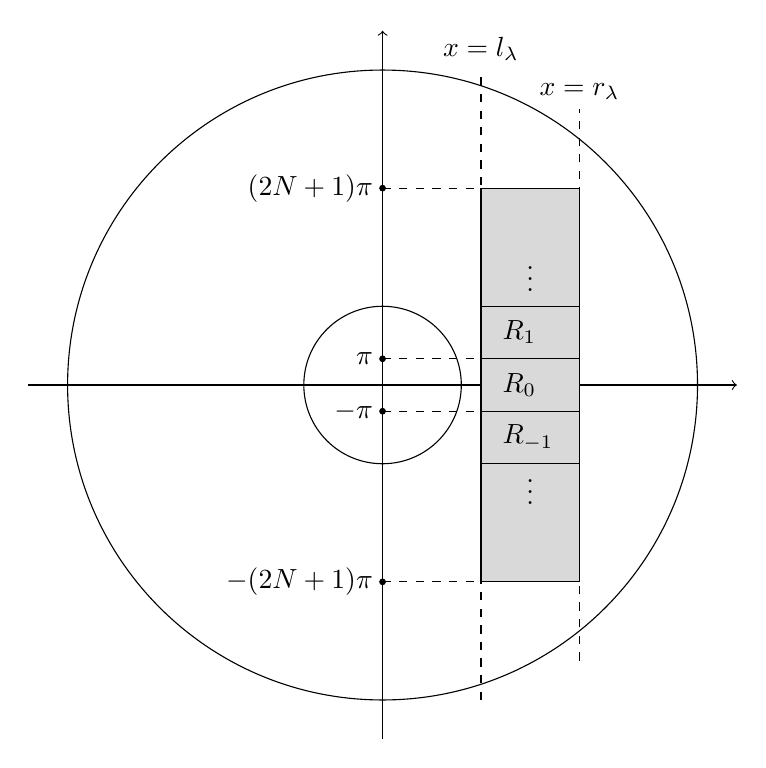
\begin{tikzpicture}
\definecolor{siva}{gray}{0.75}

\draw[->] (-4.5, 0) -- (4.5, 0);
\draw[->] (0, -4.5) -- (0, 4.5);

\draw (0, 0) circle (1);
\draw (0, 0) circle (4);

\draw[dashed] (1.25, -4) -- (1.25, 4)
node[anchor=south] {$x = l_\lambda$};
\draw[dashed] (2.5, -3.5) -- (2.5, 3.5)
node[anchor=south] {$x = r_\lambda$};

\draw[fill=gray!30] (1.25, -2.5) rectangle (2.5, 2.5);

\draw[dashed] (0, 2.5) -- (1.25, 2.5);
\draw[dashed] (0, 0.333) -- (1.25, 0.333);
\draw[dashed] (0, -0.333) -- (1.25, -0.333);
\draw[dashed] (0, -2.5) -- (1.25, -2.5);

\draw (1.25, 2.5) -- (2.5, 2.5);
\draw (1.25, 1) -- (2.5, 1);
\draw (1.25, 0.333) -- (2.5, 0.333);
% \draw[dashed] (1.25, 0) -- (2.5, 0);
\draw (1.25, -0.333) -- (2.5, -0.333);
\draw (1.25, -1) -- (2.5, -1);
\draw (1.25, -2.5) -- (2.5, -2.5);

\filldraw[black] (0, 2.5) circle (1pt)
    node[left]  {$(2N + 1) \pi$};
\filldraw[black] (0, 0.333) circle (1pt)
    node[left]  {$\pi$};
\filldraw[black] (0, -0.333) circle (1pt)
    node[left]  {$-\pi$};
\filldraw[black] (0, -2.5) circle (1pt)
    node[left]  {$-(2N + 1) \pi$};

% \draw[->] (4, 2) -- (2, 0.7);
% \draw[->] (4, 1) -- (2, 0.2);
% \draw[->] (4, -1) -- (2, -0.7);

\node[anchor=west] at (1.4, 0.67) {$R_1$};
\node[anchor=west] at (1.4, 0) {$R_0$};
\node[anchor=west] at (1.4, -0.67) {$R_{-1}$};
\node[anchor=center] at (1.875, -1.25) {$\vdots$};
\node[anchor=center] at (1.875, 1.45) {$\vdots$};

\end{tikzpicture}
    \caption{Ilustracija konstrukcije. Sivi pravokotnik je \(B (N)\).}
    \label{fig:konstrukcija}
\end{figure}
Preslikava \(E_\lambda\) desno stranico pravokotnika \(B (N)\) preslika v krožnico s središčem v izhodišču in polmerom \(\lambda e^{r_\lambda}\), medtem ko se leva stranica preslika v krog s središčem v izhodišču in radijem \(\lambda e^{l_\lambda}\). Oglejmo si kolobar
\[A = \{z : \lambda e^{l_\lambda} \leq |z| \leq \lambda e^{r_\lambda}\}.\]
Dokazali bomo, da ima \(A\) naslednji dve lastnosti.

\vspace{5mm}
\noindent \textbf{Lastnost 1}. Velja \(B (N) \subset \Int (A)\). Res, naj  bo \(z = x + i y \in B (N)\). Po definiciji \(B (N)\) imamo
\[l_\lambda \leq x \leq r_\lambda, \qquad - (2N + 1) \pi \leq y \leq (2N + 1) \pi.\]
Zato
\[|z| \leq |x| + |y| \leq r_\lambda + (2N + 1) \pi < \lambda e^{r_\lambda},\]
kar pomeni, da je \(|z|\) strogo manjše od zunanjega radija \(A\). Po drugi strani pa je
\[|z| \geq l_\lambda > \lambda e^{l_\lambda},\]
torej je \(|z|\) strogo večji od notranjega radija \(A\).

\noindent \textbf{Lastnost 2}. Funkcija \(E_\lambda\) preslika \(B (N)\) v \(A\). Res, naj bo \(z \in B (N)\). Potem \(E_\lambda (z) = \lambda e^x e^{i y}\) in zato
\[|E_\lambda (z)| = \lambda e^x \leq \lambda e^{r_\lambda} \qquad \text{in} \qquad |E_\lambda (z)| = \lambda e^x \geq \lambda e^{l_\lambda}.\]
\vspace{5mm}

\noindent Vrnemo se nazaj k konstrukciji. Za vsak \(i = -N, \dots, N\) definiramo `podpravokotnik'
\[R_i \coloneq \set{x + iy \in \CC : x \in [l_\lambda, r_\lambda], y \in [(2i - 1) \pi, (2i + 1) \pi]}.\]
Ker po lastnosti 2 \(E_\lambda\) preslika \(R_i\) v \(A\), ostaja pokazati le, je ta preslikava surjektivna. Naj bo \(w = r \lambda e^{i \theta} \in A\), torej \(r \in (e^{l_\lambda}, e^{r_\lambda})\) in \(\theta \in [(2i - 1) \pi, (2i + 1) \pi]\). Če vzamemo \(x = \ln r\) in postavimo \(z = x + i \theta\), je po definiciji \(z \in R_i\) in
\[E_\lambda (z) = \lambda e^x e^{i \theta} = \lambda r e^{i \theta} = w.\]
Tako je res \(E_\lambda (R_i) = A\). Ker to drži za vsak \(i = -N, \dots, N\), sledi tudi, da je za poljubna \(i, j\): \(R_j \subset E_\lambda (R_i)\).

Po točki (3) trditve \ref{prop:trinajst} obstaja \(\mu > 1\), da velja
\begin{equation} \label{eqn:mu-ocena}
    \bigl| E_\lambda' (z) \bigr| \geq \mu > 1 \qquad \text{na polravnini } \re z \geq l_\lambda.
\end{equation}
Zato je ta neenakost izpolnjena tudi na vsakem podpravokotniku \(R_i\). Definiramo
\[\Lambda_N \coloneq \set{z \in B(N) : E_\lambda^j (z) \in B (N) \text{ za vse } j \geq 0},\]
to je množico točk, katerih orbite pod \(E_\lambda\) ostanejo v \(B (N)\). Za vsak \(k = -N, \dots, N\) uvedemo trak
\[S (k) \coloneq \set{x + i y \in \CC : (2k - 1) \pi \leq y \leq (2k + 1) \pi}.\]
Naj bo \(L_k\) veja inverza preslikave \(E_\lambda\), definirana na pozitivno zarezani ravnini \(\CC \setminus [0, \infty)\) tako da
\[L_k (z) = \ln \prt{\frac{|z|}{\lambda}} + i \Arg_k (w),\]
kjer je \(\Arg_k (w) \in [(2k - 1) \pi, (2k + 1) \pi]\). Potem za vsak \(w \in \CC \setminus [0, \infty)\) in \(k = - N, \dots, N\) drži
\begin{equation} \label{eqn:inverz-e}
    E_\lambda \circ L_k (w) = w.
\end{equation}

\begin{trditev} \label{prop:claim}
    Za vsaka \(j, k \in \{-N, \dots, N\}\) velja \(L_k (R_j) \subset \Int (R_k)\).
\end{trditev}

\begin{dokaz}
    Ker je \(R_j \subset A\), lahko vsak \(w \in R_j\) izrazimo kot \(w = r \lambda e^{i \theta}\), kjer je \(r \in (e^{l_\lambda}, e^{r_\lambda})\) in \(\theta \in ((2k - 1) \pi, (2k + 1) \pi)\). Ker je veja inverza \(L_k\) podana z \(L_k (w) = \ln r + i \theta\) dobimo \(L_k (w) \in \Int (R_k)\).
\end{dokaz}

Za nek \(z \in \Lambda_N\) je \(\im (E_\lambda^n (z)) \neq (2j \pm 1) \pi\) za vsak \(n \in \NN\) in vsak \(j = -N, \dots, N\). Res, če je \(E_\lambda^n (z) = x + (2j \pm 1) \pi i\), potem je \(E_\lambda^{n + 1} (z) = - \lambda e^x \notin B (N)\). Zato vsaka točka \(E_\lambda^n (z)\) leži v pravokotniku
\[R_i^* \coloneq \set{x + iy \in \CC : x \in [l_\lambda, r_\lambda], y \in ((2i - 1) \pi, (2i + 1) \pi)},\]
ki ga dobimo, če pravokotniku \(R_i\) odstranimo zgornjo in spodnjo stranico. Tako vsak \(z \in \Lambda_N\) določa svoje natanko določeno zaporedje
\[\overline{s} = (s_0, s_1, s_2, \dots), \qquad s_i \in \{-N, \dots, N\}\]
za katerega velja
\begin{equation} \label{eqn:itinerar}
    E_\lambda^n (z) \in R_{s_n}^* \qquad \text{za vsak } n = 0, 1, \dots
\end{equation}
Zaporedje \(\overline{s}\) imenujemo \emph{itinerar} točke \(z\). Ker je po definiciji veje \(L_{s_n}\) za vsak \(w = E_\lambda^n (z) \in R_{s_n}^*\) prav tako \(L_{s_n} (E_\lambda (w)) = w\) sledi
\begin{equation} \label{eqn:devetpet}
    L_{s_n} \circ E_\lambda \prt{E_\lambda^n (z)} = E_\lambda^n (z).
\end{equation}

V nadaljevanju pokažemo, da za vsak \(\overline{s} \in \Sigma_N\) množica
\[\bigcap_{n \geq 0} L_{s_0} \circ \dots \circ L_{s_{n - 1}} \prt{B (N)} \coloneq \bigcap_{n \geq 1} L_s^{[n]} \prt{B (N)}\]
vsebuje natanko eno točko, ki jo označimo z \(z_{\overline{s}}\). Ker je po trditvi \ref{prop:claim} za vsak \(j, k\)
\[L_k (R_j) \subset \Int (R_k) \implies L_s^{[n + 1]} \prt{B (N)} \subset L_s^{[n]} \prt{B (N)},\]
je zaporedje množic \(\{L_s^{[n]} (B (N))\}_{n = 1}^{\infty}\) padajoče. Da je njihovo presečišče zgolj ena točka, zadostuje, da zaporedje njihovih premerov
\[d_n \coloneq \diam \prt{L_s^{[n]} \prt{B (N)}}\]
konvergira proti \num{0}. Naj bosta \(z_1, z_2 \in B(N)\). Z neenakostjo \(|E_\lambda' (z)| \geq \mu > 1\) (enačba \eqref{eqn:mu-ocena}) in enakostjo \eqref{eqn:devetpet} ter verižnim pravilom dobimo
\[\prt{L_s^{[n]}}' (z) = \prt{E_\lambda^n}' \prt{L_s^{[n]} (z)}^{-1} \implies \abs{\prt{L_s^{[n]}}' (z)} \leq \mu^{- (n + 1)}.\]
Zato
\[ \begin{multlined}[12cm]
    \left| L_s^{[n]}(z_2) - L_s^{[n]}(z_1) \right| = \left| \int_{z_1}^{z_2} \prt{L_s^{[n]}}' (z) \, \dd z \right|\\
    \leq |z_2 - z_1| \cdot \sup_{z \in B(N)}\left| \left( L_s^{[n]} \right)'(z) \right| \leq \frac{\diam (B(N))}{\mu^{n+1}}.
\end{multlined} \]
Ker je \(\mu > 1\), desna stran konvergira proti \num{0} in zato tudi \(d_n\) konvergirajo proti \num{0}.

\begin{izrek}
    Preslikava \(\phi \colon \Sigma_N \to \Lambda_N\); \(\phi (\overline{s}) = z_{\overline{s}}\) je homeomorfizem, ki konjugira skrčitev \(E_\lambda\) na \(\Lambda_N\) ter preslikavo zamika \(\sigma\). 
\end{izrek}

\begin{dokaz}
    (1) \textbf{Surjektivnost}. Naj bo \(\overline{s} \in \Sigma_N\) itinerar točke \(z \in \Lambda_N\). Z indukcijo pokažemo, da je \(\phi (\overline{s}) = z\). Za \(n = 0\) po definiciji \(z \in B (N)\) velja \(L_{s_0} \circ E_\lambda (z) = z\). Predpostavimo
    \[z = L_{s}^{[n]} \prt{E_{\lambda}^{n + 1} (z)}.\]
    Potem iz enačbe \eqref{eqn:devetpet} in verižnega pravila sledi
    \[L_{s}^{[n + 1]} \prt{E_{\lambda}^{n + 2} (z)} = L_{s}^{[n]} \prt{L_{s_{n + 1}} \circ E_\lambda (E_\lambda^{n + 1} (z))} = L_{s}^{[n]} \prt{E_\lambda^{n + 1} (z)} = z.\]
    S tem smo pokazali, da je \(z \in L_{s_0} \circ L_{s_1} \circ \dots \circ L_{s_n} (B (N))\) za vsak \(n \geq 0\) in zato \(z = \phi (\overline{s})\).

    (2) \textbf{Surjektivnost}. Naj bosta \(\overline{s}, \overline{s}^* \in \Sigma_N\), da \(\overline{s} \neq \overline{s}^*\). Naj bo \(j \in \NN\) najmanjši, da je \(s_j \neq s_j^*\). Če bi veljalo \(\phi (\overline{s}) = \phi (\overline{s}^*) = z\), bi po definiciji itinerarja veljalo
    \[E_\lambda^j (z)\in L_{s_j} \prt{B (N)} \cap L_{s_j^*} \prt{B (N)}.\]
    A za \(w \in L_{s_j} \prt{B (N)}\) je imaginarni del \(\im w \in ((2 s_j - 1) \pi, (2 s_j + 1) \pi)\), za \(w^* \in L_{s_j^*} \prt{B (N)}\) pa \(\im w^* \in ((2 s_j^* - 1) \pi, (2 s_j^* + 1) \pi)\). Ker sta ta intervala disjunktna, je to protislovje.

    (3) \textbf{Zveznost}. Naj bo \(\overline{s}^o \in \Sigma_N\) in \(z_0 = \phi (\overline{s}^o)\). Za \(\varepsilon > 0\) izberemo tak \(k\), da
    \[\frac{\diam (B (N))}{\mu^{k + 1}} < \varepsilon,\]
    kjer je \(\mu > 1\) iz ocene \(|E_\lambda'| \geq \mu\) \eqref{eqn:mu-ocena}. Potem ima vsak \(\overline{s}\) iz okolice
    \[U = \set{\overline{s} \in \Sigma_N : s_i = s_i^o \text{ za } 0 \leq i \leq k}\]
    prvih \((k + 1)\) simbolov enakih kot \(\overline{s}^o\). Tako za obe točki \(\phi (\overline{s})\) in \(\phi (\overline{s}^o)\) velja
    \[\phi (\overline{s}), \phi (\overline{s}^o) \in L_s^{[k + 1]} \prt{B (N)}.\]
    Iz neenakosti v dokazu konvergence premerov \(d_n\) tudi tukaj sledi
    \[\left| \phi (\overline{s}) - \phi (\overline{s}^o) \right| \leq \diam \prt{B (N)} \frac{1}{\mu^{k + 1}} < \varepsilon.\]
    Tako je \(\phi\) zvezna.

    (4) \textbf{Zveznost inverza}. Ker je \(\Sigma_N\) kompakten in \(\phi\) bijektivna, je \(\phi^{-1}\) zvezna.

    (5) \textbf{Konjugacija}. Če je \((s_0, s_1, s_2, \dots) = \phi^{-1} (z)\), potem je \(z \in L_s^{[n]} \prt{B (N)}\) za vsak \(n \in \NN\) in zato \(E_\lambda (z) \in E_\lambda \circ L_s^{[n]} \prt{B (N)}\) za vsak \(n \in \NN\). Uporabimo \eqref{eqn:inverz-e}, da dobimo \(E_\lambda (z) \in L_s^{[n]} \prt{B (N)}\) za vsak \(n \in \NN\). To pomeni \(E_\lambda (z) = \phi (s_1, s_2, \dots) = \phi \circ \sigma (s_0, s_1, s_2, \dots) = \phi \circ \sigma \circ \phi^{-1} (z)\).
\end{dokaz}

\noindent Končno lahko dokažemo enakost
\[\overline{\bigcup_{n \geq 1} \Lambda_N} = J (E_\lambda).\]
Po neenakosti \(|E_\lambda' (z)| \geq \mu > 1\) \eqref{eqn:mu-ocena} za vsak \(z \in \Lambda_N\) in izreku \ref{thm:julm} je \(\Lambda_N \subset J (E_\lambda)\). Ker je \(J (E_\lambda)\) zaprtje množice vseh odbojnih periodičnih točk je dovolj, da dokažemo, da je vaka taka točka v kakšni od množic \(\Lambda_N\). Naj bo \(z_0\) odbojna periodična točka preslikave \(E_\lambda\). S posledico \ref{cor:jul-e} vemo, da \(z \in \{\re z \geq l_\lambda\}\). Periodičen cikel \(\{z_0, E_\lambda (z_0), \dots\}\) je tako omeje na polravnini \(\{\re z \geq l_\lambda\}\), zato je za dovolj velik \(N\) v celoti vsebovan v \(B (N)\). Po definiciji \(\Lambda_N\) so vse točke cikla v \(\Lambda_N\), torej je tudi \(z_0 \in \Lambda_N\).



\end{document}
